\documentclass[10pt]{amsart}
\usepackage[a4paper,margin=23mm]{geometry}
\usepackage{amsmath,amssymb,amsthm,mathtools,hyperref,graphicx,xspace,letltxmacro,xpatch}
\usepackage[english]{babel}
\newtheorem{theo}{Theorem}[section]
\newtheorem{lemm}[theo]{Lemma}\newtheorem{prop}[theo]{Proposition}\newtheorem{coro}[theo]{Corollary}\newtheorem{conj}[theo]{Conjecture}
\theoremstyle{definition}\newtheorem{defi}[theo]{Definition}\newtheorem{rema}[theo]{Remark}\newtheorem{exam}[theo]{Example}\newtheorem{exem}[theo]{Example}\newtheorem{nota}[theo]{Notation}
\newcommand{\ie}{i.e.}\newcommand{\resp}{resp.}\newcommand{\skpt}{\par\smallskip\noindent}
\emergencystretch=3em\pagestyle{plain}
%~Mouliné par MaN_auto v.0.27.3 2023-10-13 11:43:47

\usepackage{mathrsfs}
\usepackage{bbm}
\usepackage{circledsteps}
\usepackage{cmap}



%\setcounter{theol}{0}
%\renewcommand*\thetheol{\Alph{theol}}
\theoremstyle{plain}
\newtheorem{theol}{Theorem}
%%\renewcommand*\thefactl{\arabic{factl}}
\renewcommand*\thetheol{\Alph{theol}}




\theoremstyle{plain}
\newtheorem{claim}{Claim}
%%\renewcommand*\thefactl{\arabic{factl}

\newcommand\BE{\approx}
\newcommand\eps{\varepsilon}
\newcommand\NLP{\Pi}
\newcommand\FNLP{\boldsymbol{\Pi}}


\newcommand\Proberg{\Prob_{\kern-3pt\mathrm{erg}}}
\newcommand\erg{\mathrm{erg}}
\renewcommand\top{{\mathrm{top}}}
\newcommand{\TV}{\mathrm{TV}}

\newcommand*\eg{{\it e.g.\ }}
\newcommand\vpot{\vec\pot}

\newcommand\dom{\operatorname{dom}}
\newcommand\inter{\operatorname{int}}
\newcommand{\wass}{\operatorname{W}}
\newcommand{\diam}{\operatorname{diam}}
\newcommand\Prob{{\operatorname{\mathscr{P}}}}
\DeclareMathOperator{\interior}{int}

\newcommand*{\dd} {\relax\ifnum\lastnodetype>0\mskip\medmuskip\fi\mathrm{d}}

\newcommand{\rs}{\operatorname{\rho}}
\newcommand{\grad}{\operatorname{\nabla}}

\newcommand{\opt}{\mathrm{opt}}

\newcommand{\hf}{\mathsf{h}}
\newcommand{\Pf}{\mathsf{P}}
\newcommand{\EM}{\mathscr{E\kern-2pt M}}

\newcommand{\pot}{\varphi}


\newcounter{In}
\newcommand{\In}{\refstepcounter{In}\Circled{\theIn}}
\newcommand{\Inref}[1]{\Circled{\ref{#1}}}
\newcommand{\phantomIn}{\refstepcounter{In}}

\renewcommand*\l{\lambda}
\newcommand*\al{\alpha}
\newcommand*\be{\beta}
\newcommand*\om{\omega}
\newcommand*\8{\infty}
\newcommand{\ol}{\overline}
\newcommand\hS{\widehat{S}}
\newcommand*\disp{\displaystyle}
\newcommand{\ninf}{{n\to+\8}}


\newcommand\NN{\mathbb{N}}
\newcommand\RR{\mathbb{R}}
\newcommand\ZZ{\mathbb{Z}}
\newcommand*\N{\mathbb{N}}
\newcommand*\R{\mathbb{R}}
\newcommand{\Z}{\mathbb{Z}}
\newcommand{\En}{\mathcal{E}}
\newcommand{\CP}{\mathcal{P}}
\newcommand{\CD}{\mathcal{D}}
\newcommand{\cD}{\mathcal{D}}
\newcommand{\CM}{\mathcal{M}}
\newcommand{\cM}{\mathcal{M}}
\newcommand{\CL}{\mathcal{L}}
\newcommand{\CG}{\mathcal{G}}
\newcommand{\cC}{\mathcal C}
\newcommand{\scY}{\mathscr{Y}}
\newcommand{\scV}{\mathscr{V}}
\newcommand{\scX}{\mathscr{X}}

\newcommand{\bfD}{\mathbf{D}}

\newcommand{\llbracket}{\mathopen{[\mkern -2.7mu[}}
\newcommand{\rrbracket}{\mathclose{]\mkern -2.7mu]}}

%%%%%%%%%%%%%%%%%%%%%%%%%%%%%%%%%%%%%%%%%%%%%%%%%%%%%%%%%%%%%%%%%%%%%%%%%%
%\newcommand\cA{\mathcal A}
%\newcommand\cB{\mathcal B}

%\newcommand\cl[1]{\left<#1\right>_\sim}
%\newcommand\cls[1]{\left<#1\right>}
%\newcommand\cG{\mathcal G}
%\newcommand\Bij{\mathfrak S}
%\newcommand\cL{\mathcal L}
%\newcommand\cM{\mathcal M}
%\newcommand\cO{\mathcal O}
%\newcommand\Class{\cC}
%\newcommand\Crit{\operatorname{Crit}}
%\newcommand\Diff{\operatorname{Diff}}

%\newcommand\embeds{{\hookrightarrow}}
%\newcommand\Fix{\operatorname{Fix}}
%\newcommand\id{\operatorname{id}}

%\newcommand\QQ{{\mathbb Q}}
%\newcommand\TT{{\mathbb T}}
%\newcommand\per{\operatorname{per}}
%\newcommand\pih{{\hat\pi}}
%\newcommand\PP{{\mathbb P}}
%\newcommand\ProbPE{{\Prob_{>0}}}
%\newcommand\rec{{\rm rec}}
%\newcommand\reg{\ast}
%\newcommand\diffsym{\operatorname{\Delta}}
%\newcommand\ret{{{\textnormal{ret}}}}
%\newcommand\BEpi{\operatorname{\stackrel\pi\BE}}
%\newcommand\simpi{\operatorname{\stackrel\pi\sim}}
%\newcommand\BEsha{\stackrel{\#}\BE}
%\newcommand\simsha{\stackrel{\#}\sim}
%\newcommand\var{\operatorname{var}}
%\newcommand\temp{\beta}
%\newcommand\supp{\operatorname{supp}}
%\newcommand*\K{{\mathbb K}}
%\renewcommand{\theenumi}{\textit{\roman{enumi}}}


%\newcommand\ffi{\varphi}
%\newcommand\fios{\varphi_{OS}}


%\newcommand*\s{\sigma}
%\newcommand*\S{\Sigma}

%\newcommand*\Om{\Omega}

%\newcommand{\wh}{\widehat}
%\newcommand{\wt}{\widetilde}
%\newcommand*\ie{{\em i.e.,\ }}
%\newcommand{\munbe}{\mu_{n,\beta}}
%\newcommand*\L{\Lambda}
%\newcommand*\l{\lambda}
%\newcommand*\te{\theta}
%\newcommand*\P{\mathbb{P}}
%\newcommand*\Q{\mathbb{Q}}
%\newcommand*\CH{\cal{H}}
%\newcommand*\mbf[1]{\mathbf{#1}}
%\newcommand*\CS{\cal{S}}

%\newcommand{\un}{{\mathbbm{1}}}
%\newcommand{\CL}{\mathcal{L}}
%\newcommand{\CM}{\mathcal{M}}


%\newcommand{\CC}{\cC}
%\newcommand{\pbqq}{{\disp h_{\mu}+\frac\be2\left(\int \psi\,d\mu\right)^{2} }}
%\newcommand{\pbq}{{\disp h_{\mu}+\left(\int \pot\,d\mu\right)^{2} }}
%\newcommand{\ul}{\underline}
%\newcommand{\uncom}{\mathbbm{1}_{[\om]}}
%\newcommand{\fibar}{\ol{\varphi}}


%\newcommand{\ga}{\gamma}
%\renewcommand{\th}{\text{th}}
%\newcommand{\argth}{\text{argth}}
%%%%%%%%%%%%%%%%%%%%%%%%%%%%%%%%%%%%%%%%%%%%%%%%%%%%%%%%%%%%%%%%%%



%%%%%%%%%%%%%%%%%%%%%%%%%%%%%%%%%%%%%%%%%%%%%%%%%%%%%%%%%%%%%%%%%%%%%%%%%%%%%%
\graphicspath{{./figures/}}

\newcommand*{\mk}{\mkern -1mu}
\newcommand*{\Mk}{\mkern -2mu}
\newcommand*{\mK}{\mkern 1mu}
\newcommand*{\MK}{\mkern 2mu}

%\hypersetup{urlcolor=purple, linkcolor=blue, citecolor=red}

\newcommand*{\romanenumi}{\renewcommand*{\theenumi}{\roman{enumi}}}
\newcommand*{\Romanenumi}{\renewcommand*{\theenumi}{\Roman{enumi}}}
\newcommand*{\alphenumi}{\renewcommand*{\theenumi}{\alph{enumi}}}
\newcommand*{\Alphenumi}{\renewcommand*{\theenumi}{\Alph{enumi}}}
\let\oldtilde\tilde
\renewcommand*{\tilde}[1]{\mathchoice{\widetilde{#1}}{\widetilde{#1}}{\oldtilde{#1}}{\oldtilde{#1}}}
\let\oldhat\hat
\renewcommand*{\hat}[1]{\mathchoice{\widehat{#1}}{\widehat{#1}}{\oldhat{#1}}{\oldhat{#1}}}
\let\oldexists\exists
\renewcommand*{\exists}{\mathrel{\oldexists}}
\let\oldforall\forall
\renewcommand*{\forall}{\mathrel{\oldforall}}
%%%%%%%%%%%%%%%%%%%%%%%%%%%%%%%%%%%%%%%%%%%%%%%%%%%%%%%%%%%%%%%%%%%%%%%%%%%%%%

\title{Variational principle for nonlinear topological pressure with continuous measure energies}
\author{Buzzi, Jérôme, Kloeckner, Benoît, Leplaideur, Renaud}
\date{doi:10.5802/ahl.192; CC BY 4.0}
\begin{document}
\maketitle
\noindent\textit{Editorial note.} Only selected author result counted; complete original mathematical body and bibliography retained. Original vector/raster figures and native TikZ retained; class frontmatter/web-only definitions omitted from rendering preamble.\par\medskip
\noindent\textit{Editorial note.} Native circledsteps dependency vendored locally from CTAN under LPPL1.3c with its copyright/license notice retained; no global installation.\par\medskip
\noindent\textit{Editorial note.} Generic wrapper eg placeholder omitted so the original author italic eg macro is used unchanged.\par\medskip
\noindent\textit{Allowed standard prerequisites (editorial).}\begin{itemize}
\item Standard functional analysis, measure theory and the author-cited classical theorems. Standard prior results stay cited; complete source-local proofs and definitions retained.
\end{itemize}\medskip



\section{Introduction}

In the 1970s, Sinai, Ruelle, Bowen, and others (see, e.g., \cite{Bowen-book,Ruelle-book,Sinai-GibbsMeasures}) developed a thermodynamical approach to dynamical systems inspired by the statistical mechanics of lattice systems. In a recent work~\cite{Leplaideur-Watbled}, the third named author and Watbled applied this program to the Curie--Weiss mean-field theory: they introduced a new thermodynamical formalism over the full shift where the energy functional is quadratic. They obtained precise results using the specific structure of this setting.

Our goal in this paper is to understand the generality of their results. It turns out that we can define the nonlinear pressure of a measure as the sum of its entropy and its ``energy'', defined as \emph{any weak-star continuous function} of the measure. We are in particular interested in the case when the energy is a smooth function of the integrals of one or several potentials, in which case we call it an \emph{energy with potential(s)}. Assuming only that the classical thermodynamical formalism is well-behaved, we can analyze this \emph{nonlinear} thermodynamics using suitable convex analysis.

First, for arbitrary continuous energies, we prove a variational principle: the supremum of the nonlinear pressure of the measures is given by a combinatorial formula involving the classical separated sets for the Bowen--Dinaburg dynamical metric (Theorem~\ref{thm-var-prin-NL}), we then define \emph{equilibrium measure} as those measures achieving the previous supremum. It is easy to show that equilibrium measures exist and, in the expansive case, we relate them to Gibbs ensembles (Theorem~\ref{thm-existence-NL}).

In the case of energies with potentials, we show that equilibrium measures are classical equilibrium measures for some specific linear combination of these potentials (Theorem~\ref{thm-equilibria}). When the nonlinearity is a real-analytic function of the integral of a single potential, we obtain finiteness of the set of equilibrium measures (Theorem~\ref{thm-finiteness}). As is well-known from physics and examples including the Curie--Weiss theory, \emph{phase transitions} can occur in this setting, e.g., there may be several equilibrium measures that may depend non-analytically on parameters giving rise to \emph{freezing} (Theorem~\ref{thm-fpt} and Section~\ref{sec:transition}) or \emph{metastable phase transitions.} (Theorem~\ref{th-metastable} in Section~\ref{sec-metastable}).

As pointed out by one of the referees, nonlinear energies have been considered in the distinct but related ``multifractal analysis'' (see Remark~\ref{r:multifractal}, and~\cite{Climenhaga2014} and the references therein for background). Theorem~\ref{thm-equilibria} is also related to constrained equilibrium measures as considered in~\cite{KW2015} and~\cite{GKLM}, see Remark~\ref{rem-max-ent-cond}.

Just prior to submitting the present version of this work, we became aware of the strongly related article~\cite{BarreiraHolanda2021}.


\subsection{Classical thermodynamical formalism}
We recall the classical definitions (see, e.g., \cite{Walters-book}). We will sometimes call these notions \emph{linear} to distinguish them from the ones we introduce in this paper.


Let $(T,\pot)$ be a continuous system, i.e., a continuous self-map $T:X\to X$ of a compact metric space together with a continuous function $\pot \in C(X,\RR)$. The function $\pot$ is called the \emph{potential}. We denote by $\Prob$ the set of Borel probability measures on $X$, endowed with the weak star topology, by $\Prob(T)$ the subset of $T$-invariant measures and by $\Proberg(T)$ the subset of ergodic and invariant measures.


The weight of order $n$ of a finite subset $\cC\subset M$ is:
\[
w_n(\cC) := \sum_{x\,\in\,\cC} \exp \left(S_n\pot(x)\right)
\]
where $S_n\pot$ denotes a Birkhoff sum:
\[
S_n\pot(x):=\pot(x)+\pot(Tx)+\dots+\pot(T^{n-1}x).
\]
Given $\eps>0$ and $n\in\NN$, the \emph{Bowen--Dinaburg dynamical balls} are the sets
\[
B(x,\eps,n):=\big\{y\in X: \forall 0\leq k<n,\; d(T^ky,T^kx)<\eps \big\}.
\]
A finite set $\cC$ is an \emph{$(\eps,n)$-covering} when $\bigcup_{x\,\in\,\cC} B(x,\eps,n)=X$. It is an \emph{$(\eps,n)$-separated} subset when for all distinct $x, x'\in \cC$, $x'\notin B(x,\eps,n)$. The \emph{partition function} is:
\[
Z(\eps,n) := \sup_{\cC} w_n(\cC)
\]
where $\cC$ ranges over the $(\eps,n)$-separated subsets of $X$.

We shall say that an $(\eps,n)$-separated set $\cC$ is \emph{adapted} when it realizes the supremum in $Z(\eps,n)$. Such sets exist since the set of $(\eps,n)$-separated subsets is closed in $X^n$ while $T$ and $\varphi$ are continuous. Each adapted set defines a probability measure
\begin{equation}
\mu_{\cC} := \frac{1}{Z(\eps,n)} \sum_{x\,\in\,\cC} e^{S_n\phi(x)} \frac{\delta_x+\delta_{Tx}+\dots+\delta_{T^{n-1}x}}{n}.
\end{equation}
called an \emph{$(\eps,n)$-Gibbs ensemble}.

The (linear) topological pressure is:
\begin{equation}\label{eq-VP-classic}
P_\top(T,\pot):=
\lim_{\eps\,\to\,0} \limsup_{n\,\to\,\infty}\frac1n\log Z(\eps,n),
\end{equation}
while the (linear) pressure of a measure $\mu\in\Prob(T)$ with respect to the potential $\pot$ is (denoting by $h$ the Kolmogorov--Sinai entropy):
\[
P(T,\pot,\mu):= h(T,\mu) + \int\pot\,d\mu.
\]
The variational principle expresses that these two notions are strongly related:
\begin{equation}\label{eq-VP}
P_\top(T,\pot) = \sup_{\mu\,\in\,\Prob(T)} P(T,\pot,\mu).
\end{equation}
An \emph{equilibrium measure} for $(T,\pot)$ is then an invariant probability measure $\mu$ such that $P(T,\pot,\mu)=P_\top(T,\pot)$, i.e., a measure that achieves the above supremum.

%\medskip
The (linear) pressure function is the function $\be\mapsto P_{\top}(T,\beta\pot)$ where $\be$ is a real parameter, called the \emph{inverse of temperature}.



\subsection{Nonlinear formalism}
We propose the following generalization. It will prove convenient to write $\mu(\pot)$ for $\int\pot \dd\mu$. We consider again a continuous map $T$ acting on a compact metric space $X$.

An \emph{energy} is a function $\En : \Prob \to \RR$ which is continuous in the weak star topology; note that we will need the energy of non-invariant measures. We say that $\En$ is an energy \emph{with potential} $\pot$ (a continuous function defined on $X$) if it can be written
\[
\En(\mu) = F\big(\mu(\pot)\big)
\]
for some continuous function $F:I\to\RR$ defined on an interval containing all values taken by $\pot$. More generally, an \emph{energy with potentials} takes the form
\begin{equation}\label{eq-Energy}
\En(\mu) = F\big(\mu(\pot_1),\,\dots,\,\mu(\pot_d)\big)
\end{equation}
where $\pot_1,\,\dots,\,\pot_d$ are continuous functions defined on $X$ and $F:U\to\RR$ is a continuous function on some set $U\subset\RR^d$. For $\En$ to be well-defined on the whole of $\Prob$, the set $U$ must contain the convex hull of the set of values taken by $\vec\pot = (\pot_1,\,\dots,\,\pot_d):X\to\RR^d$. We add the adjective ``$C^r$'' ($r\ge 1$), ``smooth'' or ``analytic'' to $\En$ whenever the domain $U$ of $F$ is open and $F$ is $C^r$ ($r=\infty$ meaning smooth, $r=\omega$ meaning analytic) on $U$.

An energy is said to be \emph{convex} when for all Borel probability measures $\xi$ on $\Prob$ (hence, $\xi$ is a measure on the set of measures):
\[
\En\left(\int \nu \dd\xi(\nu) \right) \le \int \En(\nu) \dd\xi.
\]
For example, if $\En$ is an energy with potentials, it is convex whenever $F$ is.
%\bigskip

Not assuming potentials, we first need to replace Birkhoff sums. Given $x\in X$ and $n\in\NN$, we define an \emph{empirical measure}
\[
\Delta_x^n := \frac1n \sum_{i=0}^{n-1} \delta_{T^ix}.
\]
Observe that for any potential $\pot$, $\Delta_x^n(\pot)=\frac1n S_n\pot(x)$ is the averaged Birkhoff sum. We thus define the \emph{nonlinear weight} of order $n$ of a finite set $\cC$ and the \emph{nonlinear partition function} as
\[
\omega_n(\cC) = \sum_{x\,\in\,\cC} e^{n\En(\Delta_x^n)} \qquad
\zeta(\eps,n) = \sup_{\cC} \omega_n(\cC),
\]
where the supremum is taken over all $(\eps,n)$-separated sets $\cC$.


Again, an $(\eps,n)$-separated set $\cC$ is said to be \emph{adapted} if it realizes the maximum in $\zeta(\eps,n)$ and we define an \emph{nonlinear $(\eps,n)$-Gibbs ensemble}
\begin{equation}\label{eq-def-ensemble}
\mu_{\cC} := \frac{1}{\zeta(\eps,n)} \sum_{x\,\in\,\cC} e^{n \En\left(\Delta_x^n\right)} \Delta_x^n \in\Prob
\end{equation}
(note that the continuity of $T$ ensures that the maximum in $\zeta$ is realized for all $(\eps,n)$).

The \emph{nonlinear topological pressure}, to be thought of as an analogue of topological entropy weighted by energy, is
\begin{equation}\label{eq:NLP}
\NLP_\top^\En(T) = \lim_{\eps\,\to\,0} \limsup_{n\,\to\,\infty} \frac1n \log \zeta(\eps,n).
\end{equation}
In Theorem~\ref{thm-var-prin-NL} we will show that under suitable hypotheses, replacing the supremum limit by an infimum limit:
\[
\underline{\NLP}_\top^\En(T) = \lim_{\eps\,\to\,0}\; \liminf_{n\,\to\,\infty} \frac1n \log \zeta(\eps,n)
\]
gives the same quantity as $\NLP_\top^\En(T) $. Meanwhile the \emph{nonlinear pressure} is defined for all invariant probability measures $\mu$ by
\[
\NLP^\En(T,\mu) = h(T,\mu) + \En(\mu).
\]


\subsection{Main results for general energies}

For certain nonlinear systems $(T,\En)$, it may happen that some measures satisfy $\NLP^\En(T,\mu) > \NLP_\top^\En(T)$ (see Remark~\ref{rem-vp-erg}); we will first give conditions excluding this.

\begin{defi}
We will say that $(T,\En)$ has an \emph{abundance of ergodic measures} if for any $\mu\in\Prob(T)$ and $\eps>0$, there is an ergodic measure $\nu\in \Proberg(T)$ such that { $h(T,\nu)+\En(\nu)> h(T,\mu)+\En(\mu)-\eps$}.
\end{defi}


Note that the classical property of entropy-density of ergodic measures, i.e., the existence of ergodic measures converging to $\mu$ both in the weak star topology and in entropy (see~\cite[Lemma~3.2]{FollmerOrey1988}), implies the above condition. In particular, these two conditions are satisfied by uniformly hyperbolic diffeomorphisms that have a single basic set in their spectral decomposition, and by systems with specification (see~\cite{PfisterSullivan2007}).


Arbitrary continuous systems $(T,\En)$ with convex energy have an abundance of ergodic measures (though not necessarily entropy-density of ergodicity) since, in this case, for any $\mu\in\Prob(T)$,
\[
\NLP^\En(T,\mu) \le \int \big(h(T,\mu_\xi) + \En(\mu_\xi) \big) \dd P(\xi)
\]
using the ergodic decomposition $\mu=\int \mu_\xi \dd P(\xi)$.



%\medbreak

Recall that, in the invertible case, $T$ is said to be an \emph{expansive homeomorphism} when there exists a number $\eps_0>0$ (called an \emph{expansivity constant} for $T$) such that
\[
\forall x,y\in X\quad \sup_{n\,\in\,\ZZ} d\left(T^nx,T^ny\right)\leq\eps_0 \implies x=y
\]
(see, e.g., \cite{Katok-Hasselblatt} Definition~3.2.11; note that here we use a $\le$ sign, making the expansivity constants possibly slightly smaller). This notion is generalized to not necessarily invertible maps under the name of \emph{positive expansivity} by considering only the positive orbits:
\[
\forall x,y\in X\quad \sup_{n\,\ge\,0} d\left(T^nx,T^ny\right)\leq\eps_0 \implies x=y.
\]
and the results we state below for expansive homeomorphisms could be extended to positively expansive map with the same proofs.
%\bigbreak

Our first result establishes a variational principle generalizing eq.~\eqref{eq-VP} to all energies.


\begin{theol}[Variational principle]\label{thm-var-prin-NL}
Let $T:X\to X$ be a continuous map of a compact space and let $\En:\Prob\to\RR$ be an energy. Assume that $(T,\En)$ has an abundance of ergodic measures.


Then the nonlinear topological pressure satisfies:
\begin{equation}\label{eq-def-Ptop}
\sup_{\mu\,\in\,\Prob(T)} \NLP^\En(T,\mu) = \NLP^\En_\top(T) = \underline{\NLP}_\top^\En(T).
\end{equation}
If additionally $T$ is an expansive homeomorphism with some constant $\eps_0>0$, then
\begin{equation}\label{eq-ent-eps}
\NLP^\En_\top(T) =\lim_n \frac1n \log \zeta(\eps_0,n).
\end{equation}
\end{theol}



When the conclusion $\sup_{\Prob(T)} \NLP^\En(T,\cdot) = \NLP^\En_\top(T)$ of the above theorem holds, we define a \emph{nonlinear equilibrium measure} as any measure $m\in\Prob(T)$ realizing this supremum:
\[
\NLP^\En(T,m)=\max_{\Prob(T)} \NLP^\En(T,\cdot).
\]


As in the classical setting, existence of an equilibrium measure is easily obtained when entropy is upper semicontinuous, and in the expansive case equilibrium measures prescribe the asymptotic behavior of Gibbs ensembles.

\begin{theol}\label{thm-existence-NL}
Let $T:X\to X$ be a continuous map of a compact space and let $\En:\Prob\to\RR$ be an energy. Assume that $(T,\En)$ has an abundance of ergodic measures. Then the following holds:
\begin{enumerate}\romanenumi
\item \label{enumi-B1}
If $\mu\mapsto h(T,\mu)$ is upper semicontinuous, there exists at least one nonlinear equilibrium measure.
\item \label{enumi-B2}
Under the stronger assumption that $T$ is an expansive homeomorphism for some constant $\eps_0>0$, one can be more precise: any accumulation point $\mu$ of any sequence $(\mu_{\cC_n})_{n\,\in\,\NN}$ of nonlinear Gibbs $(\eps_0,n)$-ensembles is an average of nonlinear equilibrium measures.
\end{enumerate}
\end{theol}

Note that the upper semicontinuity assumption is satisfied if $(X,T)$ is a subshift, is expansive~\cite{Walters-book} or is $C^\infty$ smooth~\cite{Buzzi-SIM}.

%\medbreak

The last statement means that there exists a probability measure $\xi$ on $\Prob$ (a measure of measures), concentrated on the set $\EM$ of equilibrium measures, such that
\[
\mu = \int_{\EM} \nu \dd\xi(\nu)
\]
(see, e.g., \cite[Proposition~1.2]{Phelps-book}) The accumulation points can indeed fail to be equilibrium measures, e.g., in the Curie--Weiss model when there are two asymmetric equilibrium measures and one chooses symmetric Gibbs ensembles, see~\cite{Leplaideur-Watbled}.

\begin{rema}\label{rem-exist-theo}
The above result is formulated in standard terms but our arguments yield a stronger result as suggested by the referee, Theorem~\ref{thm-weak-Gibbs}. Most notably, we relax upper-continuity of entropy in~\eqref{enumi-B1} and expansivity in~\eqref{enumi-B2}, replacing them by the related, but logically independent condition eq.~\eqref{eq-ent-eps}.
\end{rema}



\subsection{Main results for energies with potential}\label{subsec-energy}

Next we study the uniqueness and nature of the nonlinear equilibrium measures in the case of an energy with potentials $\vec\pot=(\pot_1,\,\dots,\,\pot_d):X\to\RR^d$ as in eq.~\eqref{eq-Energy}. Our main point here is that we can use classical convex analysis to reduce the nonlinear thermodynamical formalism to the linear one.

More precisely, we will use the classical Legendre duality between entropy and pressure; using the vector of integral of potentials $(\mu(\pot_1),\,\dots,\,\mu(\pot_d))$ as intermediate coordinates, this will reduce to finite-dimensional Legendre(--Fenchel) duality. The conditions we assume in order to apply this approach are bundled under the term ``\emph{$C^r$ Legendre} systems $(T,\vec\pot)$'' (where $r\in\NN^*\cup\{\infty,\omega\}$ and $C^\omega$ means analytic), see Definitions~\ref{defi-Legendre} and~\ref{defi-regular}. We give examples of such systems in Section~\ref{sec-examples-sys}, including classical hyperbolic systems. By Proposition~\ref{prop:nlem0} it suffices to check that the entropy is bounded and semi-continuous, that the pressure function is regular enough and strictly convex, and the following independence condition:
\begin{multline}\label{eq-independence}
\text{the convex set }\{(\mu(\pot_1),\,\dots,\,\mu(\pot_d)):\mu\in\Prob(T)\} \\
\text{ has non-empty interior in }\RR^d.
\end{multline}
Note that the failure of this condition only means that some reduction is required (see Section~\ref{subsec:potts} for an example). See also Remark~\ref{rem-livsic}.

We deduce the nonlinear equilibrium measures from the linear ones using the finite-dimensional linear pressure and entropy functions, defined as follows:
\[
\Pf(y_1,\,\dots,\,y_d) := P_\top\left(T,\sum_i y_i\pot_i \right)
\quad\text{and}\quad
\hf(z) :=\sup\left\{h(T,\mu):\mu(\vec\pot)=z\right\}
\]
for $y,z\in\RR^d$. By convention $\sup\emptyset=-\infty$. Recall the gradient $\grad\Pf:\RR^d\to\RR^d$ defined as $\grad\Pf(y_1,\,\dots,\,y_d):=(\frac{\partial\Pf}{\partial y_1},\,\dots,\,\frac{\partial\Pf}{\partial y_d})$.

\begin{theol}\label{thm-equilibria}
Assume that $(T,\vec\pot)$ is $C^{ 1}$ Legendre, that $F:U\subset\RR^d\to\RR$ is $C^{ 1}$ and consider the energy with potentials $\En(\mu) = F(\mu(\pot_1),\,\dots,\,\mu(\pot_d))$.
\begin{enumerate}\romanenumi
\item There is a nonempty compact subset $\scY\subset\RR^d$ such that the nonlinear equilibrium measures are exactly the \emph{linear} equilibrium measures with respect to each of the potentials $\sum_i y_i\pot_i$ where $(y_1,\,\dots,\,y_d)\in\scY$.

\item The set $\scY$ can be computed from the linear pressure function $\Pf$ above; more precisely,
\begin{align*}
\scY&=(\nabla \Pf)^{-1}(\scV) \text{ where }\\
\scV &=\left\{z\in\RR^d \colon \hf(z)+F(z)=\sup(\hf + F). \right\}
\end{align*}
The function $\hf$ can also be computed from $\Pf$, as $-\hf$ is the Legendre dual of~$P$.
\end{enumerate}
\end{theol}

It is possible that some potential $\sum_i y_i\pot_i$ with $(y_1,\,\dots,\,y_d)\in\scY$ admits more than one linear equilibrium measure. In this case, the theorem implies that they are all nonlinear equilibrium measures.


When a $C^r$ Legendre system $(T,\vec\pot)$ is such that each linear combination of the $(\pot_i)$ admits a unique linear equilibrium measure, one says that $(T,\vec\pot)$ is \emph{$C^r$ Legendre with unique linear equilibrium measures}. This is the case in classical hyperbolic settings. However, this does not preclude $\scY$ from containing more than one point (see, e.g., the Curie--Weiss model in Section~\ref{sec-Curie-Weiss}). Thus, under the hypotheses of Theorem~\ref{thm-equilibria}, one may have several nonlinear equilibrium measures which are all ergodic with full support and satisfy strong stochastic properties (see Corollary~\ref{cor-individual}).


\begin{rema}
Given $(T,\vpot)$ a smooth Legendre system, any compact subset of $\RR^d$ can be realized as the set $\scY$ above by choosing a suitable~$C^\infty$ smooth nonlinearity $F$ (Proposition~\ref{prop-flexibility}). In particular, in $C^\infty$ regularity, even for a single potential ($d=1$), the set of nonlinear equilibrium states can be infinite, countable or not.
\end{rema}

\begin{rema}
The proof of Theorem~\ref{thm-equilibria} applies more generally to the analysis of measures maximizing a function $G(h(T,\mu),\mu(\vec\pot))$ with $\partial G/\partial z_0>0$, see eq.~\eqref{eq-G}.
\end{rema}
%
%\bigbreak

\begin{theol}\label{thm-finiteness}
If $(T,\pot)$ is a $C^\omega$ Legendre system with unique linear equilibrium measures and $F$ is $C^\omega$ with a single potential $(d=1)$, then there are only finitely many nonlinear equilibrium measures.
\end{theol}

Note that we do not simply claim that $\EM$ is finite-dimensional, but that it is finite, even though it can contain several equilibrium measures. In fact, this failure of uniqueness can occur even for a topologically transitive subshift of finite type with a H\"older-continuous potential (see \eg~\cite{Leplaideur-Watbled} and Section~\ref{sec-examples} below). However uniqueness holds for generic non-linearities for any $d\ge1$ (Proposition~\ref{p-generic-unique}).


\subsection{Examples of \texorpdfstring{$C^r$}{Cr} Legendre systems}\label{sec-examples-sys}
%$\null$

\subsubsection{Classical hyperbolic systems}

We will say in this text that $(T,\vec\pot)$ is a \emph{classical hyperbolic system} if $T$ is a mixing subshift of finite type, a mixing Anosov diffeomorphism, or a mixing expanding map, and $\vec\pot:=(\pot_1,\,\dots,\,\pot_d)$ is a family of H\"older-continuous potentials satisfying the independence condition~\eqref{eq-independence}. Then Proposition~\ref{prop:nlem0} ensures that classical hyperbolic systems $(T,\vec\pot)$ are $C^\omega$ Legendre.

Theorem~\ref{thm-equilibria} shows that for these many systems with expanding or hyperbolic properties, the nonlinear equilibrium measures share the good ergodic properties of the classical equilibrium measures. Let us recall some of them.

\begin{coro}[Folklore]\label{cor-individual}
Let $(X,T,\vec\pot)$ be a classical hyperbolic system (not reduced to a fixed point). Consider a $C^r$ nonlinearity $F:U\subset\RR^d\to\RR$. Then, for the energy given by $\En(\mu) = F\big(\mu(\pot_1),\,\dots,\,\mu(\pot_d)\big)$, any nonlinear equilibrium measure
\begin{itemize}
\item has full support;
\item is ergodic and mixing;
\item has exponential decay of correlation;
\item satisfies the almost sure invariance principle and in particular the central limit theorem.
\end{itemize}
where the two last properties are understood to hold with respect to H\"older-con\-ti\-nuous observables.
\end{coro}

These results are folklore in the sense that some of them are immediate consequences of the founding results of Sinai, Ruelle, and Bowen, while others were first considered in more general settings. The following are convenient references: ergodicity, mixing, and exponential decay of correlation follow from Ruelle's Perron--Frobenius theorem (see, e.g.,\cite[chapter~1]{Baladi-book}), the almost sure invariance principle, which implies many limit theorems was proved in~\cite{MN05} in much greater generality.


\subsubsection{Nonuniform hyperbolic dynamics}

By construction, our approach easily applies to many nonuniformly hyperbolic systems with a suitable class of potentials. A simple example is provided by the $\beta$-shifts (see, e.g., \cite{Reniy-1957}) and H\"older-continuous potentials.


Indeed, let $(X,T)$ be the $\beta$-shift for some $\beta>1$ together with $ \varphi_1,\,\dots,\,\varphi_d:X\to\RR$ some H\"older-continuous functions satisfying the independence condition~\eqref{eq-independence}. According to~\cite[Theorem~1.2 and Example~1.5]{Climenhaga-2018-towers}, there is an irreducible countable state Markov shift $\Sigma$ with a H\"older-continuous factor map $\pi:\Sigma\to X$ such that, for every H\"older-continuous $\varphi:X\to\RR$, $(\Sigma, \varphi\circ\pi)$ is strongly positive recurrent in the sense of~\cite{Sarig-2001-PhaseTransitions} (see~\cite{Sarig-2015-thermo} for background). In particular, its Gurevič pressure coincides with the topological pressure $P_\top(T, \varphi)$. Moreover, $(\Sigma,\varphi\circ\pi)$ has a unique linear equilibrium which projects to the unique equilibrium of $(X, \varphi)$. It follows from a straightforward adaptation of~\cite{Cyr-Sarig-2009} that $\vec y\in\RR^d\mapsto P_\top(T,\vec y\cdot\vec\pot)$ is real-analytic\footnote{The cited paper only considers a single variable but the method~\cite[end of Section~3.1]{Cyr-Sarig-2009} is perfectly general and in fact also yields the real-analyticity with respect to $\vec\pot$ with the adapted norm from~\cite{Cyr-Sarig-2009}.} near each point of $\RR^d$, hence on $\RR^d$ itself. The second differential of the pressure is given by the asymptotic variance and it is positive definite under the independence condition~\cite[Theorems~6.4~and~6.5]{Sarig-2015-thermo}.



\subsubsection{Systems with a spectral gap for the transfer operator}

Another family of dynamical systems (intersecting the classical hyperbolic systems) to apply our framework to is provided by~\cite[Corollary~B, Theorems~F \& G]{GKLM}. We shall say that a Banach space $\scX$ of functions $X\to \RR$ is a \emph{good Banach algebra of functions} when:
\begin{itemize}
\item $\scX$ is stable by product and $\lVert fg\rVert \le \lVert f\rVert \lVert g\rVert$ for all $f,g\in\scX$,
\item for every positive, bounded away from $0$ function $f\in\scX$, $\log f$ is in $\scX$,
\item the norm of $\scX$ dominates the uniform norm (in particular the elements of $\scX$ are bounded),
\item the composition operator $f\mapsto f\circ T$ is a continuous operator on $\scX$,
\item for every equilibrium measure $\mu$ of a potential in $\scX$ and every non-negative $f\in\scX$, if $\int f\dd\mu = 0$ then $f=0$,
\item every continuous function can be uniformly approximated by elements of $\scX$.
\end{itemize}
(These assumptions are numerous, but many Banach spaces satisfy them, such as H\"older spaces or BV space on the interval, see~\cite{GKLM} for some discussions of these hypotheses.) We refer to~\cite{GKLM} for the notions of $k$-to-$1$ map, simple dominant eigenvalue, and spectral gap appearing in the following statement.

\begin{theo}[\cite{GKLM}]\label{thm-classical-are-Legendre}
Assume that $T$ is $k$-to-$1$ and $\pot_1,\,\dots,\, \pot_d$ belong to some good Banach algebra of functions $\scX$ and that for all $\alpha_1,\,\dots\alpha_d$ not all zero, $\sum_{i=1}^d \alpha_i\pot_i$ is not cohomologous to a constant. If for all $ y\in\RR^d$ the transfer operator defined by $\CL f (x) = \sum_{x'\,\in\,T^{-1}(x)} e^{ y\cdot\vpot(x')} f(x')$ acts with a simple dominant eigenvalue and a spectral gap on $\scX$, then $(T,\vpot)$ is $C^\omega$ Legendre with unique linear equilibrium measures.
\end{theo}



\subsection{Examples of energies}\label{subsec-examples}

We will now give a few examples of energies to which the above theorems apply, mostly inspired by physics. These examples involves an additional real parameter, the inverse temperature $\beta>0$: the energy function is then $\En(\mu)=\beta\En_1(\mu)$ where $\En_1$ is a reference energy and $\beta$ tunes the balance between entropy and that energy, in agreement with thermodynamics.\footnote{In thermodynamics, the equilibrium state of a system in contact with a thermostat at inverse temperature $\beta$ is such that it maximizes the entropy of the total system (combining the initial system and the thermostat), i.e., the quantity $h(T,\mu)-\beta\En(\mu)$, up to the addition of a constant. As is customary in dynamics, the minus sign has been included in the definition of the energy function.} This leads to the natural question of how the existence, the number, or the equilibrium measures themselves depend on this parameter $\beta$, leading to the physical notion of phase transitions.


\subsubsection{Linear case}

The classical, linear formalism is the special case where $d=1$ and $F(z)= \beta z$ for $\beta>0$ and taking any $\pot\in C(X,\RR)$. The nonlinear pressure then coincides with the linear one: $h(T,\mu)+\beta\int \pot \dd\mu$, yielding a first example. Here $\scY=\{\beta\}$.



\subsubsection{Classical Curie--Weiss model}

Consider $X=\{-1,1\}^{\NN}$ or $X=\{-1,1\}^{\ZZ}$, let $T$ be the shift map, and set $\pot(x_0x_1\cdots)=x_0$ and $F(z)=\frac\beta2z^2$ for some $\beta\ge 0$; i.e., maximize $h(T,\mu)+\frac\beta2\mu(\pot)^2$. The set $\scY$ can have one or two elements depending on the value of $\beta$: see~\cite{Leplaideur-Watbled} and Section~\ref{sec-Curie-Weiss}. { The notations were slightly different: $\NLP^\En_\top(T)$ here was $\CP_{2}(\pot)$ in~\cite{Leplaideur-Watbled}, $\hf(z)$ was $\ol{H}(z)$ and $\hf(z)+F(z)$ was $\ol\varphi(z)$.}


\subsubsection{Asymmetric Curie--Weiss model}

In Section~\ref{sec-metastable} we shall give an asymmetric Curie--Weiss model, where $T$ is again a full shift map, $\pot$ is a Bernoulli potential and $F(z)=\frac\beta2z^2$, but exhibiting a \emph{metastable} phase transition: at each temperature there are finitely many \emph{local} maximizers, but at some critical temperature the global maximizer jumps from one local maximizer to another.

\subsubsection{Curie--Weiss--Potts}

{The consideration of several potentials is motivated by} the Curie--Weiss--Potts model: $X=\{\theta_1,\,\dots,\,\theta_n\}^{\NN}$ or $X=\{\theta_1,\,\dots,\, \theta_n\}^{\ZZ}$, $T$ the shift map, $\pot_i(x_0x_1\cdots)=\mathbbm{1}_{\theta_i}(x_0)$ and $F(z)=\frac{\beta}{2} \lVert z\rVert^2$ where $\lVert\cdot\rVert$ is the usual Euclidean norm, exhibiting yet another form of phase transition as $\beta$ varies, see~\cite{Leplaideur-Watbled-2} and Section~\ref{subsec:potts}.


\subsubsection{Bethe--Peierls--Weiss approximation}\label{subsubsec-PRW}
As in the previous models, this approximation replaces the direct site-to-site interactions by an interaction with the global average, but keeps the microscopic interaction for nearest neighbors, for some parameter $0\le\alpha\le1$:
\begin{align*}
\En(\mu) &= \int_X \left(\alpha x_0 x_1 + (1-\alpha)x_0\left(\int_X y_0\,d\mu(y)\right)\right) \, d\mu(x)\\
&=\alpha \mu(x_0x_1) + (1-\alpha) \mu(x_0)^2 \\
&= F_\alpha(\mu(\vec\pot))
\end{align*}
with $F_\alpha(z_1,z_2)=\alpha z_1 +(1-\alpha) z_2^2$, $\pot_1(x):=x_0x_1$, and $ \pot_2(x)=x_0$.



\subsubsection{Mean-field energy maps}\label{subsubsec-mft}
The previous models are examples of mean field theories in statistical physics, e.g., systems of particles interacting with one another only through some \emph{averages}, the so-called molecular fields (see~\cite[Sections~10.5, 10.7]{Reif}). We translate this idea into energy maps $\En:\Prob\to\RR$ of the following form:
\begin{equation}\label{eq-mft}
\En(\mu) = \int_X V(x,\mu(\vec\pot))\, d\mu \text{ for some }\vec\pot\in C(X,\RR^d)\text{ and }V\in C(X\times\RR^d,\RR).
\end{equation}
When $V$ is linear in the averages, i.e., $V(x, z)=V_0(x)+\sum_{i=1}^d V_i(x)z_i$, this reduces to an energy with potentials with quadratic nonlinearity:
\[
\En(\mu)=\mu(V_0)+\sum_{i=1}^d \mu(V_i)\mu(\pot_i)=F(\mu(\vec\psi))
\text{ where }\vec\psi=(V_0,\,\dots,\,V_d,\pot_1,\,\dots,\,\pot_d).
\]
Note that if $(X,T)$ is the full-shift on $\{\theta_1,\,\dots,\,\theta_d\}^\ZZ$ and if we set $V_0=0$, $V_i(x)=\phi_i(x)=\sqrt{\beta/2}\cdot \mathbbm{1}_{\theta_i}(x_0)$, we get the Curie--Weiss--Potts model.

All energy maps as in eq.~\eqref{eq-mft} are continuous and thus satisfy the variational principle by Theorem~\ref{thm-var-prin-NL}. Assuming $(T,\vec\pot)$ to be a classical hyperbolic system, we further obtain the existence of equilibrium measures, and the convergence of Gibbs ensembles (Theorem~\ref{thm-existence-NL}). Finally (see Remark~\ref{rem-max-ent-cond}), any nonlinear equilibrium measure coincides with some linear equilibrium measure (inheriting its good stochastic properties, see Corollary~\ref{cor-individual}).


\subsubsection{Wasserstein distance to the maximal entropy measure}\label{sec-Wasserstein}

Let us give a simple but intriguing example going further away from energies with potentials. Consider the map $T:x\mapsto 2 x \mod 1 $ on the circle, with reference energy $\En_{1}(\mu)=\wass_p(\mu,\lambda)$ where $\lambda$ denotes the Lebesgue measure, $p\in[1,+\infty)$ and $\wass_p$ is the \emph{Wasserstein distance} of exponent $p$ (see e.g.~\cite{Villani-book}).

Theorems~\ref{thm-var-prin-NL} and~\ref{thm-existence-NL} ensure that the nonlinear topological pressure is achieved by at least one invariant measure. For $\beta=0$, $h(T,\mu)+\beta W_p(\mu,\lambda)$ reduces to the entropy so $\lambda$ is the unique equilibrium. When $\beta\to\infty$, the set of equilibrium measures must converge to $\{\delta_0\}$, since $\delta_0$ is the unique invariant measure maximizing $W_p(\mu,\lambda)$. Following a suggestion of the referee, for $p=1$ we prove in appendix that for any $\beta\in(0,+\infty)$, neither $\lambda$ nor $\delta_0$ are equilibrium measures.



\subsection{More Phase Transitions}\label{subsec-comments}
A phase transition can be defined from any of a number of different phenomena that often { occur simultaneously}: loss of the analyticity of the pressure with respect to physical parameters, multiple equilibrium measures, or failure of the central limit theorem for example.

Sarig~\cite{Sarig-2001-PhaseTransitions} has studied the equivalence of such phenomena in the setting of Markov shifts. In contrast, we see here (Section~\ref{sec-Curie-Weiss}) that non-analyticity of pressure and multiplicity of equilibrium measures can occur though the central limit theorem continues to hold (Corollary~\ref{cor-individual}). Such distinctions have been observed before in~\cite{leplaideur-butterfly} and~\cite{thaler}. The key point of view in the definition of Legendre regular systems and the proof of Theorems~\ref{thm-equilibria} and~\ref{thm-finiteness} is to consider a certain convex set, the \emph{entropy-potential diagram} (defined in Section~\ref{sec:convexity}, see Figures~\ref{fig:diagramme2D}, \ref{fig:diagramme1Da}), which describes the pairs $(h(T,\mu);\mu(\vec\pot))$ that can be achieved when $\mu$ runs over $\Prob(T)$. Phase transitions then occur when the nonlinearity ``becomes more convex'' than the diagram.

In Section~\ref{sec:transition}, we shall illustrate more broadly the benefits of this diagram by considering \emph{freezing phase transitions}, by which we mean that for all $\beta>\beta_0$ for some $\beta_0>0$, the set of equilibrium measures is non-empty and independent of $\beta$; its elements are called ``ground states'' as they must maximize the energy.

\begin{theol}\label{thm-fpt}
Let $T:X\to X$ be a continuous dynamical system of finite, positive topological entropy, and assume that $\mu\mapsto h(T,\mu)$ is upper semi-continuous.
\begin{enumerate}
\item For every $\mu_0\in\Prob_\erg(T)$ with zero entropy there exists a continuous potential $\pot:X\to \RR$ such that the \emph{linear} thermodynamical formalism of $(T,\pot)$ exhibits a freezing phase transition with unique ground state $\mu_0$.
\item For every continuous potential $\pot:X\to(-\infty,0]$ such that $K=\pot^{-1}(0)$ is $T$-invariant and has zero topological entropy, there exists a continuous nonlinearity $F : (-\infty,0]\to (-\infty,0]$ with $F(0)=0$ such that the energy $\En(\mu) = F(\mu(\pot))$ exhibits a freezing phase transition with ground states supported on $K$.
\end{enumerate}
\end{theol}

The first item is not directly related to the \emph{non-linear} thermodynamical formalism, but its analysis is a simple application of a theorem of Jenkinson~\cite{Jenkinson} and of the tools developed here (more precisely, we rely on the entropy-potential diagram introduced in Section~\ref{sec:convexity} which is central to our non-linear study).



\subsection{Questions}\label{subsec-questions}

We close this introduction with a few open questions.
\begin{itemize}
\item Without assuming abundance of ergodic measures, does a variational principle hold in \emph{restriction to ergodic} measures, that is:
\[
\sup_{\mu\,\in\,\Proberg(T)} \Pi^F(T,\pot,\mu) = \Pi^F_\top(T,\pot)?
\]
(See Remark~\ref{rem-vp-erg}.)
\item Can one find a subshift of finite type, H\"older-continuous potentials and a real-analytic nonlinearity\footnote{Recall that we ask that { real-analytic} $F$ be defined on an \emph{open} set containing the compact set of all possible values of $(\mu(\pot_1),\,\dots,\,\mu(\pot_d))$. This in particular prevents the trivial choice $F(\vec z) = -\sup\{h(T,\mu) \colon (\mu(\pot_1),\,\dots,\,\mu(\pot_d))=\vec z \}$.} such that there exist infinitely many nonlinear equilibrium measures? What if we additionally impose the quadratic nonlinearity, i.e., $F(z) = \frac12\lVert z\rVert^2$?
\item Can one find a ``natural'' energy {(necessarily not an energy with potentials) on some subshift of finite type} such that the non-linear equilibrium measure is unique but not ergodic?
\item { For the doubling map and the Wasserstein energy $W_p(\cdot,\lambda)$ from Section~\ref{sec-Wasserstein},} what can be said about the equilibrium measures for $\beta\in(0,+\infty)$, beyond Appendix~\ref{sec-appendix}?
\end{itemize}

\subsection*{Acknowledgments}

We are grateful for the referee's careful reading and pertinent suggestions that have improved this work.



\section{Variational principle and Gibbs ensembles}\label{sec-th-AB}
%\newcommand\hQ{{\widehat Q}}


In this section we prove Theorems~\ref{thm-var-prin-NL} and~\ref{thm-existence-NL}. We first introduce some convenient notations. We fix a compact metric space $X$, a map $T:X\to X$ and an energy $\En$. In order to be as general as possible, we do not assume $T$ to be continuous for now, but only Borel-measurable. Note that $X^n$ being compact, every subset is totally bounded; this ensures the finiteness of $(\eps,n)$-separated sets even when $T$ is not assumed to be continuous. We often omit $T,\En$ from the notation, i.e., $\NLP_\top = \NLP_\top^\En(T)$, $\NLP(\mu) = \NLP^\En(T,\mu)$ etc.


Recall the definitions of the empirical measures of a point $x\in X$, of the nonlinear weight of a subset $\cC\subset X$, and of the partition function:
\[
\Delta_x^n = \frac1N\sum_{k=0}^{n-1} \delta_{T^kx} \qquad
\omega_n(\cC) := \sum_{x\,\in\,\cC} e^{n\En(\Delta_x^n)} \qquad
\zeta(\eps,n) := \sup_{\mathclap{\substack{\cC \\ (\eps,n)\text{-separated}}}}\ \omega_n(\cC).
\]
Additionally, in this section we use the following notation:
\begin{align*}
\NLP_\top(\eps)&=\limsup_{n\,\to\,\infty} \frac1n \log \zeta(\eps,n) &
\text{so that }\NLP_\top &= \lim_{\eps\,\to\,0} \NLP_\top(\eps) \\
\underline{\NLP}_\top(\eps) &= \liminf_{n\,\to\,\infty} \frac1n \log \zeta(\eps,n) &\underline{\NLP}_\top &= \lim_{\eps\,\to\,0} \underline{\NLP}_\top(\eps).
\end{align*}


%\bigskip

Theorem~\ref{thm-var-prin-NL} starts with the equalities:
\begin{equation}\label{eq-def-Ptop1}
\sup_{\mu\,\in\,\Prob(T)} \NLP(\mu) = \NLP_\top = \underline{\NLP}_\top.
\end{equation}
under two hypotheses, continuity of $T$ and abundance of ergodic measures without which some partial results still hold. We decompose the proof in a sequence of inequalities: \phantomIn\label{In:1}
\phantomIn\label{In:2}
\phantomIn\label{In:3}
\phantomIn\label{In:4}
\addtocounter{In}{-4}
\begin{equation}\label{eq-var-ppl}
\sup_{\mu\,\in\,\Proberg(T)} \NLP(\mu)
\underset{\tiny\In}{\leq} \underline{\NLP}_\top
\underset{\tiny\In}{\leq} \NLP_\top
\underset{\tiny\In}{\leq} \sup_{\mu\,\in\,\Prob(T)} \NLP(\mu)
\ \underset{\tiny\In}{\leq}\sup_{\mu\,\in\,\Proberg(T)} \NLP(\mu).
\end{equation}
Inequality $\Inref{In:1}$ is proved in Proposition~\ref{prop:upper-ergodic} without either hypotheses and Inequality $\Inref{In:2}$ immediately follows from the definitions of $\NLP_\top$ and $\underline{\NLP}_\top$. Inequality $\Inref{In:4}$ is proved in Proposition~\ref{prop-ine probproberg} assuming an abundance of ergodic measures but without needing $T$ to be continuous. Finally, Inequality $\Inref{In:3}$ is proved in Section~\ref{sec:Gibbs}, Proposition~\ref{prop-lower-bound} assuming that $T$ is continuous, without needing an abundance of ergodic measures.

The last part of Theorem~\ref{thm-var-prin-NL} (expansive case) is proved in Section~\ref{sec-Th-A-expansive}, and the first part of Theorem~\ref{thm-existence-NL} (existence of equilibrium measures) in Lemma~\ref{lemm-existence}.



\begin{rema}\label{rem-vp-erg}
If $(T,\En)$ is continuous but without an abundance of ergodic measures, the following example shows that inequality
\[
\NLP_{\top} <\sup_{\mu\,\in\,\Prob(T)} \NLP(\mu)
\]
may hold.


Let $(X,T)$ be the union of two distinct fixed points $p,q$. Let $\En(\mu) = F(\mu(\pot))$ with $F(z)=-z^2$, $\pot(p)=1$, $\pot(q)=-1$. Then $\NLP(\mu)=0$ for $\mu=\frac12(\delta_p+\delta_q)$ whereas $\NLP_\top=-1$.
\end{rema}



\subsection{Preliminaries}

We will use the Wasserstein distance of exponent $1$ on the set $\Prob$ of probability measures on $X$. Proofs of the statements we need can be found in many places, e.g., \cite{Villani-book}.

The distance between $\mu_1,\mu_2\in\Prob$ can be defined as
\[
\wass(\mu_1,\mu_2) = \sup \big\{\mu_1(f)-\mu_2(f) \colon f \text{ $1$-Lipschitz function } X\mapsto \RR \big\}.
\]
The ``Kantorovich duality'' states that this definition is equivalent to
\[
\wass(\mu_1,\mu_2) = \inf \left\{\int d(x,y) \dd \pi(x,y) \colon \pi\in\Gamma(\mu_1,\mu_2) \right\}
\]
where $d$ is the distance on $X$ and $\Gamma(\mu_1,\mu_2)$ is the set of `transport plans'', i.e., Borel probability measures on $X\times X$ with marginals $\mu_1$ and $\mu_2$. Moreover in these definitions both the supremum and the infimum are reached; a transport plan realizing the Wasserstein distance is said to be \emph{optimal}. The compactness of $X$ implies that the Wasserstein distance induces the weak-star topology on $\Prob$, and that Wasserstein distance can be bounded above by total variation distance:
\[
\wass(\mu_1,\mu_2) \le \diam(X) \left\lVert \mu_1-\mu_2\right\rVert_{\TV}
\]

We will also use the following reformulation of Birkhoff's ergodic theorem.

\begin{lemm}\label{l:Birkhoff}
Let $\mu\in\Prob(T)$ be ergodic. Then for $\mu$-almost all $x\in X$, we have $\Delta_x^n \to \mu$ in the weak-star topology.
\end{lemm}

\begin{proof}
Let $(f_k)_{k\,\in\,\NN}$ be a dense sequence of the space $C(X,\RR)$ of continuous functions $X\to\RR$, endowed with the uniform norm. There exists a set $E$ {with $\mu(E)=1$} such that for all $x\in E$ and all $k\in\NN$, $\Delta_x^n(f_k) \to \mu(f_k)$ as $n\to\infty$.

Let $f\in C(X,\RR)$ and $\eps>0$. There exist $k\in\NN$ such that $\lVert f-f_k\rVert_\infty \le \eps$, and $N\in\NN$ such that for all $n\ge N$ and all $x\in E$, $\lvert \Delta_x^n(f_k)-\mu(f_k)\rvert\le\eps$. We then have $\lvert \Delta_x^n(f)-\mu(f)\rvert \le 3\eps$.
\end{proof}


\subsection{Bounding below the nonlinear topological pressure}

We prove Inequality $\Inref{In:1}$, then Inequality $\Inref{In:4}$ {assuming an abundance of ergodic measures.} Note that continuity of $T$ is not needed at this stage.

\begin{prop}[Inequality \Inref{In:1}]\label{prop:upper-ergodic}
Recall that $X$ is a compact metric space. If $T:X\to X$ is Borel-measurable, then for all \emph{ergodic} $\mu\in\Prob(T)$, we have $\NLP(\mu)\le \underline{\Pi}_\top$.
\end{prop}

\begin{proof}
Consider any $\gamma>0$. Since $\En$ is continuous and $\Prob$ is compact, $\En$ is uniformly continuous: there exists $\delta>0$ such that for all $\nu\in\Prob$, $\wass(\nu,\mu)\le 2\delta \implies \En(\nu)\ge \En(\mu)-\gamma$.

By the Brin--Katok entropy formula~\cite{Brin-Katok}, taking $\delta$ small enough we can also ensure that there exist $B\subset X$ with $\mu(B)\ge \frac34$ and $M_B\in\NN$ such that for all $x\in B$ and all $n\ge M_B$ we have
\[
\Big\lvert \frac1n \log \mu(B(x,2\delta,n)) + h(T,\mu) \Big\rvert \le \gamma.
\]

By Lemma~\ref{l:Birkhoff}, there are a set $A\subset X$ with $\mu(A)\ge\frac34$ and $M_A\in\NN$ such that for all $x\in A$ and all $n\ge M_A$ we have $\wass(\Delta_x^n,\mu)\le \delta$.



Consider any $n\ge\max(M_A,M_B)$ and any $0<\varepsilon\le\delta$. Let $\cC$ be any $(\varepsilon,n)$-separated set of $X$ that is maximal with respect to inclusion; in particular, $\cC$ is an $(\eps,n)$-cover, hence a $(\delta,n)$-cover. Let $\cC'$ be a minimal subset of $\cC$ that is an $(\delta,n)$-cover of $A\cap B$.

On the one hand, for all $x\in \cC'$ by minimality $B(x,\delta,n)$ intersects $B$; picking any $y$ in the intersection, we get $\mu(B(x,\delta,n)) \le \mu(B(y,2\delta,n)) \le e^{n(\gamma-h(T,\mu))}$. Since $\mu(A\cap B)\ge \frac12$, it follows
\[
\lvert \cC'\rvert \ge \frac12 e^{n(h(T,\mu)-\gamma)}.
\]

On the other hand, for all $x\in \cC'$ by minimality $B(x,\delta,n)$ intersects $A$; picking any $y$ in the intersection, we have $\wass(\Delta_y^n,\mu)\le \delta$ and $d(T^i x,T^iy)\le \delta$ for all $i\in \{0,\,\dots,\linebreak n-1\}$. By considering the transport plan $\sum_i \frac1n \delta_{T^i x} \otimes \delta_{T^i y}$, we see that $\wass(\Delta_x^n,\Delta_y^n)\le \delta$. The triangular inequality then ensures $\wass(\Delta_x^n,\mu)\le 2\delta$, and we get
\[
\En(\Delta_x^n)\ge \En(\mu)-\gamma.
\]

Using these two inequalities, we get
\[
\omega_n(\cC) \ge \omega_n(\cC') \ge \lvert \cC'\rvert \min_{x\,\in\,\cC'} e^{n\En\left(\Delta_x^n\right)} \ge \frac12 e^{n\left(h(T,\mu)-\gamma\right)} e^{n\left(\En(\mu)-\gamma\right)} \ge \frac12 e^{n\left(\NLP(\mu)-2\gamma\right)}.
\]
Since $\cC$ is $(\eps,n)$-separated, we get
\[
\frac1n \log\zeta(\eps,n) \ge \NLP(\mu)-2\gamma -\frac1n \log 2.
\]
Taking the infimum limit as $n\to\infty$, we obtain that for all $\gamma>0$, there exists $\delta>0$ such that for all $\varepsilon\in(0,\delta)$:
\[
\underline{\NLP}_{\top}(\varepsilon)\ge \NLP(\mu)-2\gamma,
\]
and letting $\eps$ then $\gamma$ go to zero ends the proof.
\end{proof}

Observe that we only used lower-semicontinuity for $\En$ here; but its upper-semicontin\-uity ensures it reaches its supremum, a desirable feature. This motivates the continuity requirement in the definition of an energy.



\begin{prop}[Inequality $\Inref{In:4}$]\label{prop-ine probproberg}
If $T$ is Borel-measurable and $(T,\En)$ has an abundance of ergodic measures, then $\sup_{\mu\,\in\,\Prob(T)} \NLP(\mu) \le\sup_{\mu\,\in\,\Proberg(T)} \NLP(\mu)$.
\end{prop}


\begin{proof}
Let $\mu$ be any invariant probability measure.
{Since} $(T,\En)$ has an abundance of ergodic measures, there is a sequence of measures $\nu_n\in\Proberg(T)$ such that { $\lim_{\ninf} h(T,\nu_n)+\En(\nu_n) \ge h(T,\mu)+\En(\mu)$}; this yields that
\[
h(T,\mu)+\En(\mu) \le \sup_{\nu\,\in\,\Proberg(T)} \NLP(\nu)
\]
holds for every $\mu$ in $\Prob(T)$.
\end{proof}



\subsection{Bounding from above the nonlinear topological pressure}\label{sec-Gibbs}

To conclude the proof of equality~\eqref{eq-def-Ptop}, it remains to prove Inequality $\Inref{In:3}$ by constructing measures almost realizing the nonlinear topological pressure. To any $(\varepsilon,n)$-separated set $\cC$, we associate the measure
\begin{equation}\label{eq-muC}
\mu_{\cC} = \frac{1}{\omega_{n}(\cC)} \sum_{x\,\in\,\cC} e^{n\En\left(\Delta_x^{n}\right)} \Delta_x^{n}.
\end{equation}
Here no assumption is made on the value of $\omega_{n}(\cC)$; if it happens $\omega_n(\cC)=\zeta(\varepsilon,n)$, then $\mu_{\cC}$ is a non-linear Gibbs ensemble. By considering a sequence of Gibbs ensembles, we will obtain $\Inref{In:3}$ (Proposition~\ref{prop-lower-bound}) and the second part of Theorem~\ref{thm-existence-NL}, which we will generalize by considering general $\mu_{\cC}$ (Theorem~\ref{thm-weak-Gibbs}).

The first step is to decompose $(\varepsilon,n)$-separated sets $\cC$ into pieces ``carrying almost constant energy''.

\begin{theo}\label{thm-Gibbs}
Assume that $T$ is continuous and consider $\varepsilon>0$, an increasing sequence of positive integers $(n_k)_k$ and a sequence of $(\varepsilon,n_k)$-separated sets $\cC_k$ such that $\frac{\log \omega_{n_k}(\cC_k)}{n_k}$ converges.

Then there exist partitions $\bfD_k=(\cD_{k,i})_{1\,\le\,i\,\le\,N_k}$ of $\cC_k$ and $I_k\subset \llbracket 1,N_k\rrbracket$ non-empty sets with the following properties:
\begin{enumerate}\romanenumi
\item\label{enumi-Gibbs-i}
for every sequence $(i_k)_k \in\prod_k I_k$, every accumulation point $\mu_\infty$ of $(\mu_{\cD_{k,i_k}})_k$ is $T$-invariant and
\[
\NLP(\mu_\infty) \ge \lim_k \frac{\log \omega_{n_k}(\cC_k)}{n_k},
\]
\item\label{enumi-Gibbs-ii}
As $k\to\infty$,
\[
\sum_{i\,\in\,\llbracket 1,N_k\rrbracket\setminus I_k} \omega_{n_k}(\cD_{k,i}) = o\big(\omega_{n_k}(\cC_k) \big)
\]
\end{enumerate}
\end{theo}

Observe that the generalized Gibbs ensemble associated to $\cC_k$ decomposes as a convex combination of the generalized Gibbs ensemble associated to each element of the partition:
\[
\mu_{\cC_k} = \sum_{i\,\in\,I_k} \frac{\omega_{n_k}(\cD_{k,i_k})}{\omega_{n_k}(\cC_k)} \mu_{\cD_{k,i_k}} + \sum_{i\,\in\,\llbracket 1,N_k\rrbracket\setminus I_k} \frac{\omega_{n_k}(\cD_{k,i_k})}{\omega_{n_k}(\cC_k)} \mu_{\cD_{k,i_k}}.
\]
The subsets $\cD_{k,i}$ are the pieces of ``almost constant energy'' mentioned above, and the exponential growth of $\omega_{n_k}(\cC_k)$ makes it possible to separate ``good'' subsets ($i\in I_k$), \emph{each} having about the same growth than $\cC_k$, and ``bad'' subsets, which \emph{together} amount for a negligible part of the mass.

Note that the measures $\frac{1}{\lvert \cD_{k,i} \rvert} \sum_{x\,\in\,\cD_{k,i}} \Delta_x^{n_k}$ could be preferred for the proof of \Inref{In:3}, and can be treated in pretty much the same way


We control the entropy using Misiurewicz' proof of the variational principle~\cite{Misiurewicz-VP}, from which we extract the following result:

\begin{lemm}[Misiurewicz]\label{lem-Misiurewicz}
Let $(\cD_k)_{k\,\in\,\NN}$ be a sequence of $(\eps,n_k)$-separated sets where $n_k\to\infty$. Assume that for each $k$, $\sigma_k$ is a probability measure concentrated on $\cD_k$ (with arbitrary weights) and that
\[
\mu_k = \frac{1}{n_k}\sum_{\ell=0}^{n_k-1} T_*^\ell \sigma_k
\]
converges in the weak star topology to some measure $\mu_\infty$.

Fix any finite partition $\alpha$ of $X$ into subsets of diameter less than $\eps$ and with negligible boundaries with respect to $\mu_\infty$ {(such an $\alpha$ always exists). Then} for all $m\in\NN$,
\[
H_{\mu_k}(\alpha^m) \ge \frac{m}{n_k} H_{\sigma_k}(\alpha^{n_k})-\frac{2m^2}{n_k}\log\lvert\alpha\rvert \qquad \forall k \text{ such that }n_k\ge 2m
\]
and $H_{\mu_k}(\alpha^m)\to H_{\mu_\infty}(\alpha^m)$ as $k\to\infty$.
\end{lemm}

Here $H_{\mu}(\al)$ stands for the entropy for the measure $\mu\in \Prob(T)$ of the partition $\al$. The proof is not reproduced here, let us simply mention that it consists in partitioning in $m$ different ways the integer interval $\llbracket 0, n_k-1\rrbracket$ into subintervals of length $m$ plus a small remainder at the start and end. Note that the hypothesis that $ \cD_k$ is $(\eps,n_k)$-separated is intended to make the computation of $H_{\sigma_k}(\alpha^{ n_k})$ a formality: each element of $\alpha^{ n_k}$ contains at most one element of $ \cD_k$.

%\bigskip
\begin{proof}[Proof of Theorem~\ref{thm-Gibbs}.]
Recall that we assume $T$ to be continuous and consider a fixed $\varepsilon>0$, some increasing sequence $(n_k)$, and $(\varepsilon,n_k)$-separated sets $\cC_k$ and assume that $\frac{\log \omega_{n_k}(\cC_k)}{n_k}$ converges to some $\ell\ge 0$.

\begin{lemm}
There exists a sequence of positive real numbers $\gamma_k\to 0$ such that for each $k$ we can cover $\Prob$ by a certain number $N_k$ of balls with fixed radius (for the Wasserstein distance) on each of which the energy $\En$ varies by at most $\gamma_k$. Moreover we can choose $(\gamma_k)_k$ and $(N_k)_k$ such that $\big\lvert\log\frac{\gamma_k}{N_k}\big\rvert=o(n_k)$.
\end{lemm}

\begin{proof}
First we set $(N_k)_k$ as any sequence that goes to infinity sub-exponentially in $n_k$, e.g. $N_k=n_k$. Since $\Prob$ is compact, we can find $(r_k)_k$ tending to $0$ such that for all $k$, $N_k$ balls of Wasserstein radius $r_k$ suffice to cover $\Prob$. Since $\En$ is continuous on the compact set $\Prob$, it is uniformly continuous and we can find $(\gamma_k')_k$ tending to $0$ such that
\[
\forall k,\forall \mu,\nu\in\Prob,\quad \wass(\mu,\nu)\le 2r_k \implies \lvert \En(\mu)-\En(\nu)\rvert < \gamma_k'.
\]
It suffices to set $\gamma_k=\max\{\gamma_k',1/N_k\}$.
\end{proof}

We fix sequences $(\gamma_k)_k$ and $(N_k)_k$ as above.

\begin{lemm}\label{lem-dividing}
For each $k$, there exist numbers $(E_i)_{1\,\le\,i\,\le\,N_k}$, a partition $\bfD_k=(\cD_{k,i})_{1\,\le\,i\,\le\,N_k}$ of $\cC_k$ and $I_k\subset \llbracket 1,N_k\rrbracket$ such that
\begin{enumerate}\romanenumi
\item\label{lemm2.8.1} $\sum_{i\,\notin\,I_k}\omega_{n_k}(\cD_{k,i})\le \gamma_k \omega_{n_k}(\cC_k)$,
\item\label{lemm2.8.2} for all $i\in I_k$, $\omega_{n_k}(\cD_{k,i})\ge \frac{\gamma_k}{N_k} \omega_{n_k}(\cC_k)$,
\item\label{enumi:dividing3}
for all $i$, for all $\mu\in\Prob$ that is a convex combination of the measures $\Delta_x^{n_k}$ where $x$ runs over $\cD_{k,i}$, $\lvert \En(\mu)-E_i\rvert < \gamma_k$.
\end{enumerate}
\end{lemm}

\begin{proof}
Fix $k$ and let $r>0$ and $S=\{\mu_1,\,\dots,\,\mu_{N_k}\}$ be such that the balls with center in $S$ and radius $r$ cover $\Prob$, and such that $\lvert\En(\mu)-\En(\mu_i)\rvert<\gamma_k$ for all $\mu\in B(\mu_i,r)$. Set $E_i : =\En(\mu_i)$, and for each $\mu\in\Prob$ define $i(\mu) = \min\{i \mid \wass(\mu,\mu_i)\le r_k\}$. Then the $V_i=\{\mu\in \Prob\mid i(\mu)=i\}$ form a partition of $\Prob$, and for all $\mu\in V_i$ we have $\lvert \En(\mu) - E_i\rvert \le \gamma_k$.

For each $i$, let $\cD_{k,i} = \{x\in \cC_{k} \mid \Delta_x^{n_k}\in V_i\}$. Let $I_k$ be the set of indices $i$ such that $\omega_{n_k}(\cD_{k,i})\ge \frac{\gamma_k}{N_k} \omega_{n_k}(\cC_k)$; the first two items follow directly from this definition.

Consider a probability measure $\mu= \sum_{x\,\in\,\cD_{k,i}} a_x \Delta_x^{n_k}$; then $\wass(\mu,\mu_i)\le r$: indeed, we have for each $x\in \cD_{k,i}$ a coupling $\pi_x\in\Gamma(\Delta_x^{n_k},\mu_i)$ of cost at most $r$, and the cost of the coupling $\sum_x a_x \pi_x\in\Gamma(\mu,\mu_i)$ is thus at most $r$. As a consequence, $\lvert \En(\mu)-E_i\rvert \le \gamma_k$.
\end{proof}

Item~\eqref{enumi-Gibbs-ii} in the theorem follows directly from $\sum_{i\notin I_k}\omega_{n_k}(\cD_{k,i})\le \gamma_k \omega_{n_k}(\cC_k)$ and $\gamma_k\to 0$. We now prove item~\eqref{enumi-Gibbs-i}: let $(i_k)_k \in \prod_k I_k$ be a sequence of ``good'' indices and set $\mu_k = \mu_{\cD_{k,i_k}}$. Up to passing to a further subsequence, we assume $\mu_\infty=\lim_k \mu_k$; since $\lvert \En(\mu_k)-E_{i_k}\rvert < \gamma_k$, it follows that $E_{i_k} \to \En(\mu_\infty)$.

To check that $\mu_\infty\in\Prob(T)$, first observe that $\wass(\Delta_x^{n_k},T_*\Delta_x^{n_k})\le \frac{\diam X}{n_k}$ by the total variation bound and conclude using an averaged coupling as in the proof of Lemma~\ref{lem-dividing} above that $\wass(\mu_k,T_*\mu_k)\to 0$. The continuity of $T$ ensures that $T_*\mu_k\to T_*\mu_\infty$, and we get $\wass(\mu_\infty,T_*\mu_\infty)=0$, i.e., $\mu_\infty\in\Prob(T)$.

Consider a partition $\alpha$ of $X$ whose elements have diameter at most $\eps$ and whose boundaries have zero measure with respect to $\mu_\infty$. Setting
\[
\sigma_k = \frac{1}{\omega_{n_k}(\cD_{k,i_k})} \sum_{x\,\in\,\cD_{k,i_k}} e^{n_k \En\left(\Delta_x^{n_k}\right)}\delta_x
\]
we have $\mu_k= \frac{1}{n_k} \sum_{j=0}^{n_k-1} T_*^j \sigma_k$. Since $\cD_{k,i}$ is $(\eps,n_k)$-separated,
\begin{align*}
H_{\sigma_k}(\alpha^{n_k}) &= \sum_{x\,\in\,\cD_{k,i_k}} p_x \log\frac{1}{p_x} \qquad\text{where } p_x = \frac{e^{n_k \En\left(\Delta_x^{n_k}\right)}}{\omega_{n_k}(\cD_{k,i_k})} \\
&= \frac{1}{\omega_{n_k}(\cD_{k,i_k})} \sum_{x\,\in\,\cD_{k,i_k}}e^{n_k \En\left(\Delta_x^{n_k}\right)} \big(\log \omega_{n_k}(\cD_{k,i_k}) -n_k\En\left(\Delta_x^{n_k}\right)\big) \\
&\ge \frac{1}{\omega_{n_k}(\cD_{k,i_k})} \sum_{x\,\in\,\cD_{k,i_k}}e^{n_k \En\left(\Delta_x^{n_k}\right)} \big(\log \omega_{n_k}(\cC_{k})+\log\frac{\gamma_k}{N_k} -n_k E_{i_k} -n_k\gamma_k\big) \\
&= \log \omega_{n_k}(\cC_{k})+\log\frac{\gamma_k}{N_k} -n_k E_{i_k} -n_k\gamma_k.
\end{align*}
Applying Lemma~\ref{lem-Misiurewicz} to $\cD_{k,{i_k}}$, for all $m\in\NN$ and all $k$ such that $n_k\ge 2m$:
\begin{align*}
H_{\mu_k}\left(\alpha^{m}\right)\ge m\left(\frac{\log \omega_{n_k}(\cC_{k})}{n_k}+ \frac1{n_k}\log\frac{\gamma_k}{N_k} - E_{i_k} -\gamma_k\right) -\frac{2m^2}{n_k}\log\lvert\alpha\rvert.
\end{align*}
Letting $k\to\infty$, then $m\to \infty$:
\begin{align*}
\frac 1m H_{\mu_k}(\alpha^{m}) &\ge \lim_k \frac{\log \omega_{n_k}(\cC_{k})}{n_k} -\En(\mu_\infty) \\
\NLP(\mu_\infty) &\ge \lim_k \frac{\log \omega_{n_k}(\cC_{k})}{n_k}.
\end{align*}
\end{proof}

Theorem~\ref{thm-Gibbs} will be reused later on, but already provides us with inequality \Inref{In:3}:

\begin{prop}\label{prop-lower-bound}
If $T$ is continuous, then we have $\sup_{\mu\in\Prob(T)} \NLP(\mu) \ge \NLP_\top$.
\end{prop}

\begin{proof}
Let $\delta>0$ and choose $\varepsilon>0$ such that $\NLP_\top(\varepsilon)>\NLP_\top-\delta$. Consider a sequence $\cC_k$ of $(\varepsilon,n_k)$-separated sets such that $\log\frac{\omega_{n_k}(\cC_k)}{n_k} \to \NLP_\top(\varepsilon)$. Apply Theorem~\ref{thm-Gibbs} and consider any sequence $i_k\in I_k$ and any accumulation point $\mu_\infty$ of $(\mu_{\cD_{k,i_k}})$. Then $\NLP(\mu_\infty)\ge \NLP_\top(\varepsilon)>\NLP_\top-\delta$.
\end{proof}


Assuming $T$ is continuous and an abundance of ergodic measures, we have shown that:
\[
\NLP_\top \le \sup_{\mu\,\in\,\Prob(T)} \NLP(\mu) \leq \underline{\NLP}_\top.
\]
Since, obviously, $\underline{\NLP}_\top \le \NLP_\top$, the above inequalities must be equalities. This proves eq.~\eqref{eq-def-Ptop1} under the assumptions of Theorem~\ref{thm-var-prin-NL}.


\subsection{Proof of Theorem~\ref{thm-var-prin-NL}: the expansive case}\label{sec-Th-A-expansive}

We assume that $T$ is a homeomorphism admitting the expansivity constant $\eps_0>0$. To begin with, we let $0<\eps\le\eps_0$ and show that
\begin{equation}\label{eq-Ptop-exp0}
\NLP_\top(\eps)=\NLP_\top(\eps_0):=\limsup_{n\,\to\,\infty} \frac1n\log\zeta(\eps_0,n).
\end{equation}

Let us prove that $\NLP_\top(\eps)\leq\NLP_\top(\eps_0)$ by extracting an $(\eps_0,n)$-separated set from an $(\eps,n)$-separated one and comparing their weights.

We first fix $\gamma>0$ arbitrarily small. By the uniform continuity of $\En$ on $\Prob$, there is $0<\delta \leq2\eps$ such that
\begin{equation}\label{eq-ECU}
W(\mu,\nu)<\delta\implies \lvert \En(\mu)-\En(\nu) \rvert<\gamma.
\end{equation}

We need the following version of the Theorem of uniform expansivity.
\begin{claim}
There exists $N\geq1$ such that for all $n\geq 2N$, for any $x\in X$,
\begin{equation}\label{eq-expansivity}
\forall N\leq k<n-N\quad \diam\left(T^k(B(x,\eps_0,n))\right)<\delta/2 \leq\eps.
\end{equation}
\end{claim}

\begin{proof}[Proof of the Claim]
If this does not hold, pick for every $N$ : $n_{N}\ge 2N$, $N\le k_{N}\le n_{N}-N$ and $x_{N}$ such that
\[
\diam\left(T^{k_{N}}(B(x_{N},\eps_{0},n_{N}))\right)\ge \delta/2.
\]
Pick $N_{0}$ and $N\ge N_{0}$. Note the following inclusions:
\begin{multline*}
B\left(T^{k_{N}}(x_{N}),\eps_{0}, N_{0}\right)\supset B\left(T^{k_{N}}(x_{N}),\eps_{0}, N\right)\\
\supset B\left(T^{k_{N}}(x_{N}),\eps_{0}, n_{N}-N\right)\supset T^{k_{N}}(B(x_{N},\eps_{0},n_{N})).
\end{multline*}


Then, consider any accumulation point $y$ for $y_{N}:=T^{k_{N}}(x_{N})$. This yields
\[
\forall N_{0},\ \diam(B(y,\eps_{0},N_{0}))\ge \delta/2.
\]
This is in contraction with the fact that $\eps_{0}$ is an expansivity constant.
\end{proof}

We now fix some finite $(\eps/2,N)$-cover $C_\eps$ of $X$ and some large enough integer $n\geq1$ (exactly how large will be specified later on; in particular we assume equation~\eqref{eq-expansivity} holds).


Given an arbitrary nonempty $(\eps,n)$-separated subset $S$ of $X$, we consider $\hS$ any $(\eps_0,n)$-separated subset of $S$, maximal for inclusion.

\begin{claim}\label{claim-W}
The following facts hold for all large $n$:
\begin{enumerate}\romanenumi
\item\label{itemNotEmpty}
For every $x\in S$, $B(x,\eps_0,n)\cap \hS$ is nonempty;
\item\label{itemCloseEnergy}
For every $x\in S$ and every $y\in B(x,\eps_0,n)$, $\lvert \En(\Delta^n_x)-\En(\Delta^n_y) \rvert \leq \gamma $.
\item\label{itemBounded}
For every $y\in \hS$, $1\le \lvert B(y,\eps_0,n)\cap S \rvert \le \lvert C_\eps\rvert^2$;
\end{enumerate}
\end{claim}

\begin{proof}[Proof of the claim]
To see that~\eqref{itemNotEmpty} holds, note that, if for some $x\in S$, $B(x,\eps_0,n)\cap \hS=\emptyset$, $\hS\cup\{x\}$ would still be $(\eps_0,n)$-separated, contradicting the maximality of $\hS$.

To prove~\eqref{itemCloseEnergy}, let $x,y$ be any two points of $X$ with $y\in B(x,\eps_0,n)$. By eq.~\eqref{eq-expansivity}, $d(T^kx,T^ky)<\delta/2$ for all $N\leq k<n-N$, hence we get:
\[
\begin{aligned}
W\left(\Delta^n_x,\Delta^n_y\right) &\leq \frac1n\sum_{k=0}^{n-1} d\left(T^kx,T^ky\right)
\leq \frac{2N}{n}\diam(X) + \frac\delta2 <\delta
\end{aligned}
\]
for large enough $n$. The claim~\eqref{itemCloseEnergy} now follows from eq. \eqref{eq-ECU}.

We turn to~\eqref{itemBounded}. Since $\hS\subset S$, $y\in B(y,\eps_0,n)\cap S$ so this set is not empty. To prove the upper bound let $I:B(y,\eps_0,n)\cap S\to C_\eps\times C_\eps$ satisfy $I(z)=(w,w')$ with $w\in B(z,\eps/2,N)$ and $w'\in B(T^{n-N}z,\eps/2,N)$. Observe that such a map exists since $C_\eps$ is a $(\eps/2,N)$-cover of $X$ and let us check that $I$ is injective. Indeed, let $z,z'\in B(y,\eps_0,n)\cap S$ with $I(z)=I(z')=:(w,w')$ and note:
\begin{itemize}
\item for all $0\leq k<N$, $d(T^kz,T^kz')\leq d(T^kz,T^kw)+d(T^kw,T^kz') <\eps$;
\item for all $N\leq k<n-N$, $d(T^kz,T^kz') < \eps$ from eq.~\eqref{eq-expansivity};
\item for all $n-N\leq k<n$,
\[
d\left(T^kz,T^kz'\right)\leq d\left(T^kz,T^{k-(n-N)}w'\right)+d\left(T^{k-(n-N)}w',T^kz'\right) <\eps.
\]
\end{itemize}
Thus $z,z'\in S$ are not $(\eps,n)$-separated and thus must be equal, proving the injectivity of the map $I$, proving~\eqref{itemBounded}. Claim~\ref{claim-W} is established.
\end{proof}


We now compare the weights of $S$ and $\hS$:
\begin{align*}
\omega_n(\hS) &= \sum_{y\,\in\,\hS} e^{n\En\left(\Delta^n_y\right)}
\geq \sum_{y\,\in\,\hS} \min_{x\,\in\,B(y,\eps_0,n)\cap S} e^{n\En\left(\Delta^n_x\right)} &\text{since }\hS\subset S\\
&\geq \sum_{y\,\in\,\hS} \frac{e^{-\gamma n} }{\left\lvert B(y,\eps_0,n)\,\cap\,S\right\rvert} \sum_{x\,\in\,B(y,\eps_0,n)\,\cap\,S} e^{n\En\left(\Delta^n_x\right)} &\text{ by eq. \eqref{itemCloseEnergy}}\\
&\geq \sum_{y\,\in\,\hS} \frac{e^{-\gamma n}}{\left\lvert C_\eps\right\rvert^2} \sum_{x\,\in\,B(y,\eps_0,n)\cap S} e^{n\En\left(\Delta^n_x\right)} &\text{ by eq. \eqref{itemBounded}}\\
&\geq \frac{e^{-\gamma n}}{\lvert C_\eps\rvert^2} \sum_{x\,\in\,S} \left\lvert B(x,\eps_0,n)\cap\hS\right\rvert \, e^{n\En\left(\Delta^n_x\right)} & \text{exchanging the sums}\\
&\geq \frac{e^{-\gamma n}}{\lvert C_\eps\rvert^2} \omega_n(S) &\text{ by eq.~\eqref{itemNotEmpty}}.
\end{align*}
Therefore, $\frac1n\log\zeta(\eps_0,n)\geq \frac1n\log\omega_n(\hS)\geq\frac1n\log\zeta(\eps,n)-\gamma-\frac1n\log\lvert C_\eps\rvert^2$. Hence,
\[
\Pi_\top(\eps):=\limsup_{n\to\infty}\frac1n\log\zeta(\eps,n)\leq \limsup_{n\to\infty}\frac1n\log\zeta(\eps_0,n)+\gamma=:\Pi_\top(\eps_0)+\gamma
\]
as $\gamma>0$ was arbitrary we obtain: $\NLP_\top(\eps)\leq\NLP_\top(\eps_0)$ for all $0<\eps\leq\eps_0$. The definitions immediately yield the inequality $\zeta(\eps_0,n)\leq\zeta(\eps,n)$ and therefore $\NLP_\top(\eps)=\NLP_\top(\eps_0)$. This proves~\eqref{eq-Ptop-exp0}.



The same argument applies to $\underline{\NLP}_\top(\eps):=\liminf_{n\,\to\,\infty}\frac1n\log\zeta(\eps,n)$ yielding: $\underline{\NLP}_\top(\eps)\linebreak = \underline{\NLP}_\top(\eps_0)$. By eq.~\eqref{eq-def-Ptop1}, $\lim_{\eps\to0} \NLP_\top(\eps)= \lim_{\eps\,\to\,0} \underline{\NLP} _\top(\eps)$. Thus, $\NLP_\top(\eps)= \underline{\NLP} _\top(\eps)$ for all $0<\eps\leq\eps_0$: the upper and lower limits of $\frac1n\log\zeta(\eps,n)$ as $n$ goes to $\infty$ coincide. Thus, we have a true limit, independently of $\eps\in(0,\eps_0)$:
\[
\NLP_\top = \lim_{n\,\to\,\infty} \frac1n\log\zeta(\eps,n),
\]
concluding the proof of Theorem~\ref{thm-var-prin-NL}.


\subsection{Existence of an equilibrium measure and convergence of the Gibbs ensembles}\label{sec:Gibbs}

We now prove Theorem~\ref{thm-existence-NL}; first its existence claim is a simple consequence of the variational principle we just established as Theorem~\ref{thm-var-prin-NL}.

\begin{lemm}\label{lemm-existence}
Assume that $T$ is continuous with $\mu\mapsto h(T,\mu)$ upper semi\-conti\-nuous, and that $(T,\En)$ has an abundance of ergodic measures. Then the set $\EM$ of nonlinear equilibrium measures is non-empty and compact.
\end{lemm}

\begin{proof}
By assumption $\mu\mapsto h(T,\mu)+\En(\mu)$ is upper semi-continuous on the compact set $\Prob(T)$, it must therefore reach its maximum on a non-empty compact set. By Theorem~\ref{thm-var-prin-NL}, that maximum is $\NLP^\En_\top(T)$ and therefore that set is $\EM$.
\end{proof}

The second part of Theorem~\ref{thm-existence-NL} follows from Theorem~\ref{thm-Gibbs}; we are actually in a position to prove the following more general result, applicable beyond the expansive case.


\begin{theo}\label{thm-weak-Gibbs}
Assume that $T$ is continuous, that $(T,\En)$ has an abundance of ergodic measures, and that there exists $\eps>0$ such that $\NLP_\top(\varepsilon) = \NLP_\top$.

Let $(\cC_k)_k$ be a sequence of $(\varepsilon,n_k)$-separated subsets of $X$ where $n_k\to\infty$, such that:
\begin{equation}
\frac{\log(\omega_{n_k}(\cC_k))}{n_k} \to \limsup_{n\,\to\,\infty}\frac1n\log\zeta(\eps,n) =:\NLP_\top(\varepsilon).\label{eq-aGibbs}
\end{equation}
Then any limit measure of $(\mu_{\cC_k})_k$ can be written as an average of nonlinear equilibrium measures.
\end{theo}

Observe in particular that we do not require entropy to be semi-continuous, and that the conclusion implies, nonetheless, existence of equilibrium measures. It seems that this relaxation of the usual hypothesis had not been noticed before even in the linear thermodynamical formalism, and we thank again the referee for pointing it out.


\begin{proof}
Consider a sequence of $(\varepsilon,n_k)$-separated sets $\cC_k$ such that $\log\frac{\omega_{n_k}(\cC_k)}{n_k} \to \NLP_\top(\varepsilon) = \NLP_\top$. Let $\mu_\infty$ be an accumulation point of $(\mu_{\cC_k})_k$, and up to extracting a further subsequence assume $\mu_\infty = \lim_k \mu_{\cC_k}$. Apply Theorem~\ref{thm-Gibbs} to write
\[
\mu_{\cC_k} = \sum_{i\,\in\,I_k} a_i \mu_{\cD_{k,i}} + \rho_k
\]
where $a_i = \frac{\omega_{n_k}(\cD_{k,i})}{\omega_{n_k}(\cC_k)}$ and $\rho_k$ is a positive measure whose total mass goes to $0$. Set
\[
b_i=\frac{a_i}{\sum_{j\,\in\,I_k} a_j}, \qquad \mu_k= \sum_{i\,\in\,I_k} b_i \mu_{\cD_{k,i}};
\]
then $\mu_k$ is a probability measure and by the total variation bound, $\wass(\mu_k,\mu_{\cC_k})\to0$, so that $\mu_k\to\mu_\infty$.

Define a sequence of probability measures over $\Prob$ (i.e. measures of measures) by
\[
\eta_k=\sum_{i\,\in\,I_k} b_i \delta_{\mu_{\cD_{k,i}}}
\]
where $\delta_\mu$ is the Dirac mass at $\mu\in\Prob$, so that we can rewrite $\mu_k$ as an integral: $\mu_k=\int \mu\dd\eta_k(\mu)$. Up to a further extraction, since the space $\Prob^{(2)}$ of measures of measures is compact in the weak-star topology induced by the weak-star topology of $\Prob$, we can assume that $\eta_k$ converges to some $\eta\in \Prob^{(2)}$. Then
\[
\mu_\infty = \lim_k \int \mu \dd\eta_k(\mu) = \int \mu \dd\eta(\mu).
\]
Now, every measure $\mu$ lying in the support of $\eta$ is an accumulation point of a sequence $(\mu_{\cD_{k,i_k}})_k$ where $(i_k)_k\in\prod_k I_k$, and is thus invariant with $\NLP(\mu) \ge \lim_k \log\frac{\omega_{n_k}(\cC_k)}{n_k} = \NLP_\top$, i.e. $\mu$ is an equilibrium measure.
\end{proof}



\section{Convexity and nonlinear equilibrium measures}\label{sec:convexity}

In this section, which is independent of Section~\ref{sec-th-AB}, we prove Theorem~\ref{thm-equilibria}, i.e., we study the nonlinear formalism for an energy with potentials. Specifically, we consider a continuous map $T:X\to X$ with finite entropy $h_\top(T)<\infty$ together with an energy defined as
\[
\En(\mu) = F\big(\mu(\pot_1),\,\dots,\,\mu(\pot_d)\big)
\]
for all $\mu\in\Prob(T)$ where, for some positive integer $d$,
\begin{itemize}
\item $\pot_1,\,\dots,\,\pot_d:X\to\RR$ are continuous functions called the \emph{potentials};
\item $F:U\to\RR$ is a smooth function called the \emph{nonlinearity}.
\end{itemize}

Here we assume that $U\subset\RR^d$ is an open set containing the compact and convex \emph{rotation set}
\[
\rs(\pot_1,\,\dots,\,\pot_d) := \big\{\big(\mu(\pot_1),\,\dots,\,\mu(\pot_d)\big) \colon \mu\in\Prob(T) \big\}.
\]
It will sometimes be convenient to write the potentials as a single vector-valued function $\vpot := (\pot_1,\,\dots,\,\pot_d)$ with the notation
\[
\vpot(x) := (\pot_1(x),\,\dots,\,\pot_d(x)), \quad \mu(\vpot):=(\mu(\pot_1),\,\dots,\,\mu(\pot_d))\quad \text{etc.}
\]
We are going to study the nonlinear equilibrium measures:
\[
\EM := \big\{\mu\in\Prob(T):h(\mu)+F(\mu(\vpot))\text{ is maximal}\big\}
\]

\begin{rema}
If one would like to apply the general results from Section~\ref{sec-th-AB} (the variational principle of Theorem~\ref{thm-var-prin-NL} and the equidistribution of Gibbs ensembles of Theorem~\ref{thm-existence-NL}), then one should demand $\En(\mu)$ to be defined for all (not necessarily invariant) probability measures, i.e., the open set $U$ should contain the convex hull of $\{\vpot(x):x\in X\}$.
\end{rema}


The rest of this section is divided as follows. First, we introduce a simple but central object, the \emph{entropy-potential diagram}, then consider a ``fully nonlinear formalism'' which is the natural setting of our technique. Second we recall the relevant background concerning Legendre duality and we set up appropriate definitions to use this duality and we provide examples of dynamical systems satisfying them. Thirdly we weave all this together and apply Legendre duality in the dynamical context to achieve the main goal of this section, Theorem~\ref{thm:equilibria-G} (which contains Theorem~\ref{thm-equilibria}). Finally we deduce some uniqueness results (Corollary~\ref{cor-finite-1D}, Propositions~\ref{p-generic-unique}~and~\ref{prop-flexibility}).



\subsection{The entropy function and the entropy-potential diagram}

Our method will boil down to finite-dimensional convex duality; to this end, we consider a reduction of the entropy (introduced in Section~\ref{subsec-energy}) and an associated domain of $\RR^{d+1}$.

\begin{defi}\label{defi-entropy}
Given a continuous dynamical system $T$ with potentials $\vpot$, the \emph{(finite-dimensional) entropy function} $\hf:\RR^d\to\RR\cup\{-\infty\}$ is\footnote{The usual convention $\sup(\varnothing) = -\infty$ is understood.}
\[
\hf(z) := \sup_{\mu\,\in\,\cM(z)} h(T,\mu).
\]
The \emph{entropy-potential diagram} is the hypograph of the entropy function:
\[
\cD = \big\{ (z_0;z_1,\,\dots,\,z_d) \in [0,+\infty) \times \RR^d \colon \exists \mu\in \Prob(T),\; h(T,\mu)\ge z_0,\;\forall i,\;\mu(\pot_i)=z_i\big\}.
\]
\end{defi}

Under our standing assumptions ($X$ compact, $\vpot$ continuous, and $h_\top(T)<\infty$), we have $\{z\in\RR^d:\hf(z)\ne-\infty\}=\rs(\vpot)$. Since the Kolmogorov-Sinai entropy is affine, $\cD$ is a convex set (see Figure~\ref{fig:diagramme2D}), i.e., $\hf$ is concave.

\begin{figure}
\centering
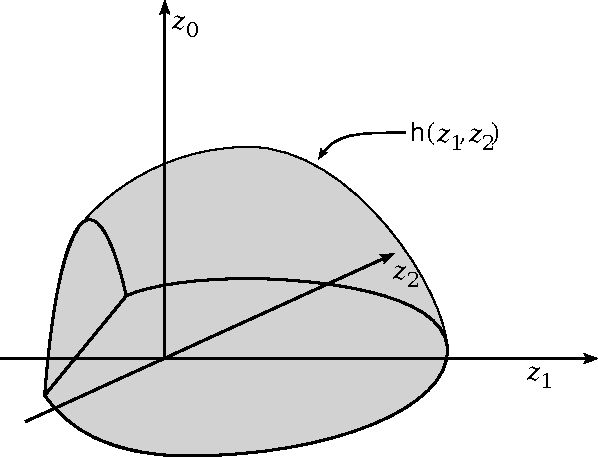
\includegraphics[scale=1]{diagramme2D.pdf}
\caption{An entropy-potential diagram in two dimensions (first coordinate represented by the vertical axis), in a case when the rotation set is not strictly convex.}\label{fig:diagramme2D}
\end{figure}

The linear pressure associated to any linear combination $\sum_i y_i \pot_i$ can be recovered from $\cD$ by finding the unique\footnote{Since we fix the normal vector, uniqueness here does not depend on smoothness of $\cD$; it is the contact points that may be non-unique, if strict convexity is not assumed.} support hyperplane with normal vector $(1;y_1,\,\dots,\linebreak y_d)$; this has important consequences, see Proposition~\ref{prop:nlem}. Let us show in a simple case how one can use $\cD$.


\begin{prop}\label{prop-interior}
Let $\mu_0\in\Prob(T)$ be such that $z=(z_1,\dots, z_d)=\mu_0(\vec \varphi)$ lies in the interior of $\rs(\vec \varphi)$ and maximizing entropy among all $\mu\in\Prob(T)$ such that $\mu(\vec\varphi)=z$. Then $\mu_0$ is a linear equilibrium measure for some linear combination $\sum_i y_i \pot_i$.
\end{prop}

\begin{proof}
Let $H$ be a support hyperplane of $\cD$ at the point $(z_0=h(T,\mu_0), z_1,\,\dots,\linebreak z_d)$. If $H$ where vertical, it would contain the point $(0,z_1,\,\dots,\,z_d)$; since $\{0\}\times \rs(\vec \varphi)$ is on one side of $H$, $z$ would be on the boundary of $\rs(\vec \varphi)$ which is precluded by hypothesis. Thus $H$ is not vertical, and the lower half-space $H^-$ it bounds is defined by an inequation of the form $(x_0+\sum y_i x_i \le c)$, where $(x_i)_{0\,\le\,i\,\le\,d}$ are the coordinates on $\RR^{d+1}$ and $y_1,\,\dots,\,y_d,c$ are some real numbers. Since $(z_0,z_1,\,\dots,\,z_d)$ is on $H$, we have $c=h(T,\mu_0)+\sum y_i\mu_0(\varphi_i) = h(T,\mu_0)+\mu_0(\sum y_i\varphi_i)$. Now for every $\mu\in\Prob(T)$, we have $(h(T,\mu),\mu(\varphi_1),\dots,\mu(\varphi_d))\in \cD \subset H^-$, so that $h(T,\mu) + \mu(\sum y_i\varphi_i) \le h(T,\mu_0)+\mu_0(\sum_i y_i\varphi_i)$, as claimed.
\end{proof}



\begin{rema}
To maximize $\hf+F$ amounts to find the largest $k$ such that there exists $ z\in\rs(\vpot)$ at which $\hf(z) = -F(z)+k$, i.e., to find the highest vertical translate of the graph of $-F$ that touches the entropy-potential diagram. One essential point of the proof of Theorem~\ref{thm-equilibria} will be to show that the touching points are located above the \emph{interior} of the rotation set, and this is where the $C^r$ Legendre assumption and the differentiability of $F$ will play a role. Then Proposition~\ref{prop-interior} shows that nonlinear equilibrium measures will correspond to linear equilibrium measures associated to one or several linear combinations of potentials, whose coefficients are given by the equations of the support hyperplanes at the touching points, see, e.g., Figure~\ref{fig:CurieWeiss} p.~\pageref{fig:CurieWeiss}.
\end{rema}


\begin{rema}\label{r:multifractal}
As pointed out by the referee, the entropy-potentials diagram and the function $\hf$ are intimately related to the multifractal formalism, more precisely to the study of the function $z \mapsto h(T|K_z)$ where $h$ is the topological entropy restricted to the subset
\[
K_z := \left\{x\in X \,\middle|\, \lim_n \frac1n\sum_{i=0}^{n-1}\vec\varphi\left(T^i x\right) = z \right\}
\]
Indeed, under suitable assumptions a \emph{conditional variational principle} holds~\cite{BarreiraSaussolSchmeling2002}:
\[
h(T|K_z) = \max\big\{ h(T,\mu) \,\big|\, \mu(\vec\varphi) = z \big\} = \hf(z)
\]
and this function was observed to be Legendre dual to a pressure, a fact we will use below. We also refer to~\cite{PfisterSullivan2007,TakensVerbitskiy2003} where more general maps and potentials are considered. Other references include~\cite{BarreiraSaussol2001,Climenhaga2013,Olivier1998}, and~\cite{Olsen2003}. The ``non-linear deformations of empirical measures'' in this later work are close to our energies; the use of duality we present here might thus allow to tackle this non-linear framework using linear methods. The multifractal formalism suggests considering energies $\En(\mu)=\frac{\mu(f)}{\mu(g)}$ for positive functions $f, g$ on $X$.
\end{rema}



\subsection{Fully nonlinear pressure}
Our approach to the energies with potentials actually applies to the following more general setting:

\begin{defi}\label{def-fully-nonlin}
Given a continuous system $T$ with potentials $\vpot$, a \emph{fully nonlinear pressure} is a function
\begin{equation}\label{eq-G}
\FNLP^G(\mu,\vpot) := G\big(h(\mu); \mu(\pot_1),\,\dots,\,\mu(\pot_d)\big)
\end{equation}
defined for all $\mu\in\Prob(T)$ {by} some smooth $G:V \to\RR$ assumed to be \emph{admissible}: it is defined on an open subset $V$ of $\RR\times\RR^{d}$ and satisfies:\footnote{The notation $\partial_0G$ refers to $\partial G/\partial z_{0}$, the derivative with respect to the first variable, corresponding to entropy since the coordinates are numbered as $(z_0,z_1,\,\dots,\,z_d)$.}
\[
\partial_0G>0
\text{ and } V\supset\left\{(h(T,\mu),\mu(\pot_1),\,\dots,\,\mu(\pot_d)):\mu\in\Prob(T)\right\}.
\]
The corresponding set of \emph{fully nonlinear equilibrium measures} is then:
\[
\EM(T,G,\vpot) := \left\{\mu\in\Prob(T):\FNLP^G(\mu,\vpot)\text{ is maximal }\right\}.
\]
\end{defi}

We will reduce the problem of maximizing $\FNLP^G$ to the classical, linear thermodynamical formalism by justifying the following claims:
\begin{itemize}
\item[$(\ast)$] given ${z}\in\rho(\vpot)$, maximizing $\FNLP^G$ and maximizing the linear pressure over
\[
\cM(z):=\{\mu\in\Prob(T):\mu(\vpot)= z\}
\]
are both equivalent to maximizing the entropy there;
\item[$(\ast\ast)$] the values $z=\mu(\vpot)$ realized by fully nonlinear equilibrium measures $\mu$ belong to the interior of rotation set $\rs(\vpot)$;
\item[$(\ast\ast\ast)$] there is a diffeomorphism $\operatorname{int}(\rho(\vpot))\to\RR^d$, ${z}\mapsto{y}$, such that, for every ${z}\in\operatorname{int}(\rho(\vpot))$, there is a linear equilibrium measure $\nu_{ y}$ for the potential
\[
{y}\cdot\vpot:=\sum_j y_j\pot_j
\]
with $\nu_y(\vpot)= z$.
\end{itemize}
The first point is immediate given the assumption that $\partial_0 G>0$. The second and third point will follow from some convex analysis; the second point more precisely follows from the assumption that the gradient of entropy diverges at the boundary in the definition of $C^r$ Legendre systems (Definitions~\ref{defi-regular} and~\ref{defi-Legendre}), see the proof of Theorem~\ref{thm:equilibria-G}.


\subsection{Legendre duality}


To apply the well-rounded theory of Legendre duality, let us introduce its classical assumptions, following~\cite{Rockafellar-book}.

We consider convex functions $f:\RR^d\to\RR\cup\{ +\infty\}$ that are proper, i.e., not identically $+\infty$ (\cite[p.~24]{Rockafellar-book} excludes the value $-\infty$). The \emph{Legendre transform} $f^*$ of $f$ is:
\[
f^*:\RR^d\to\RR\cup\{+\infty\},\quad y \mapsto \sup_{x\,\in\,\RR^d} \big(y \cdot x - f(x)\big).
\]


We also consider concave functions $g:\RR^d\to\RR\cup\{ -\infty\}$ that are proper, i.e., not identically $-\infty$. We define their Legendre transforms:
\[
g^{\#}:\RR^d\to\RR\cup\{ +\infty\},\quad y \mapsto \sup_{x\,\in\,\RR^d} \big(y \cdot x + g(x)\big),
\]
i.e., $g^{\#}:=(-g)^*$, which is convex.\footnote{Sometimes, the Legendre transform of a concave function is defined as $-(-g)^*$ instead, so that it is again concave.}
For a convex or concave function $f$, we define the \emph{(effective) domain} to be the set of points $\dom(f)$ in $\RR^d$ where it takes a finite value: $\dom(f)=f^{-1}(\RR)$.\footnote{The definition~\cite[p.~23]{Rockafellar-book} coincides for proper functions.}



%\medbreak

We will use two classical duality results from~\cite{Rockafellar-book}. They ensure that the Legendre transform is an involution on suitable classes of semicontinuous or smooth convex functions.

%\medbreak

\subsubsection*{Semicontinuous functions}
We have the following classical duality~\cite[Corollary~12.2.1]{Rockafellar-book}.


\begin{theo}\label{theo-duality-CO}
The Legendre transform maps bijectively the class of upper semicontinuous,\footnote{Convex (resp. concave) functions that are lower (resp. upper) semicontinuous are called (\emph{closed} in~\cite[p.~52]{Rockafellar-book}).} proper concave functions to the class of lower semicontinuous proper convex functions. Moreover, this restriction of the Legendre transform is an involution up to sign: for all such $f$, $f=-(f^{\#})^*$.
\end{theo}

The above theorem implies that the Legendre transform is an involution over the class of lower semicontinuous proper convex functions $g$ : $(g^*)^*=g$.


\subsubsection*{Smooth functions} 
We consider the smoothness classes $C^r$ for $1\leq r\leq\omega$, i.e., for any positive integer $r$ as well as $r=\infty$ (infinitely differentiable) and $r=\omega$ (real-analytic). The following abuses of notation will be convenient: for $r=\infty$ or $\omega$, $C^{r-1}$ just means $C^r$; for $r=0$, a $C^r$ diffeomorphism is a homeomorphism.

We adapt the definition of a concave Legendre function from~\cite[Chapitre~23]{Rockafellar-book}.

\begin{defi}\label{defi-Legendre}
A concave function $f:\RR^d\to\RR\cup\{-\infty\}$ is said to be \emph{concave of $C^r$ Legendre type} for some $1\leq r\leq\omega$ when the following conditions are satisfied:
\begin{enumerate}\romanenumi
\item\label{item-c0}
the function $f$ is upper semicontinuous;
\item\label{item-c1}
the interior $\inter\dom(f)$ is not empty and, on this set, $f$ is strictly concave and $C^r$ smooth; when $r\geq2$, we additionally ask that the Hessian of $f$ is everywhere negative definite;
\item\label{item-c2}
for all sequences $(x_i)_{i\,\in\,\NN}$ with $x_i\in\inter(\dom(f))$ which converge to a boundary point of $\dom(f)$,
\[
\lim_i \left\lvert \grad f(x_i) \right\rvert = +\infty.
\]
\end{enumerate}
We say that a function $g:\RR^d\to\RR\cup\{+\infty\}$ is convex of $C^r$ Legendre type if $-g$ is concave of $C^r$ Legendre type.
\end{defi}

Note that this notion implies properness and that, if $r=1$, it defines exactly the convex functions of Legendre type in the sense of Rockafellar~\cite[Chapitre~26]{Rockafellar-book}. Note also that the condition~\eqref{item-c2} is vacuous when $\dom(f)=\RR^d$.


Let us now state some consequences from the classical theory of Legendre duality.

\begin{theo}\label{theo-Legendre}
For each $1\leq r\leq\omega$, the Legendre transform of any concave function $f$ of $C^r$ Legendre type is a convex function $f^\#$ of $C^r$ Legendre type. Moreover, the following holds:
\begin{enumerate}\romanenumi
\item\label{theo3.9.1} $ -\grad f:\inter(\dom(f))\to\inter(\dom(f^\#))$ is a $C^{r-1}$-diffeomorphism;
\item\label{enumi:duality}
for all $y\in\inter(\dom(f^\#))$, $\grad f^\# (y) = (\grad f)^{-1}(-y)$ and
\[
f^\#(y)=z\cdot y+f(z) \text{ for a unique }z=(\grad f)^{-1}(-y);
\]
\item\label{theo3.9.3} $(f^{\#})^*=-f$.
\end{enumerate}
\end{theo}


If $f$ is a convex $C^r$ Legendre function, the above applies to $-f$: the transform $f^*=(-f)^\#$ is convex of $C^r$ Legendre type with the same properties except for minus signs: the diffeomorphism in~\eqref{theo3.9.1} is $\grad f:\inter\dom(f)\to\inter(\dom(f^*))$; in~\eqref{enumi:duality}, $y\in\inter(\dom(f^*))$ and $\grad f^*(y)=(\grad f)^{-1}(y)$, $f^*(y)=z\cdot y-f(z)$ and $z=(\grad f)^{-1}(y)$; in~\eqref{theo3.9.3} $f^{**}=f$.


\begin{proof}
This statement follows from the results in~\cite[Chapitre~26]{Rockafellar-book}, except for the formula for $f^\#(y)$ in~\eqref{enumi:duality}. When $r=1$, this is exactly Theorem~26.5 there applied to the convex function $g=-f$. Indeed, $f^\#=g^*$ and $\grad f = I\circ\grad g$ with $I(y)=-y$. In particular, $\grad g^* = (\grad g)^{-1}$, i.e., $\grad f^\# = (I\circ\grad f)^{-1} =(\grad f)^{-1}\circ I$, proving the first formula in claim~\eqref{enumi:duality}.

Now, $\grad f$ is a $C^{r-1}$ map. From the same theorem, $\grad f:\dom(f)\to\dom(f^\#)$ is a homeomorphism. It is a $C^{r-1}$-diffeomorphism, using, if $r\geq2$, that the Hessian of $f$ is definite. The formula for $\grad f^\#$ ensures that this gradient is also $C^{r-1}$, thus $f^\#$ is~$C^r$.

To conclude, let $y\in\inter(\dom(f^\#))$. Note that $ z := (\grad f)^{-1}(-y)\in\inter(\dom(f))$ satisfies $\grad_{ z}\,(y\cdot z+f(z))=0$. Since $f$ is strictly concave on $\inter(\dom(f))$ and concave everywhere, $ z$ must be the unique maximizer on $\dom(f)$, proving the second half of~\eqref{enumi:duality}.
\end{proof}

\subsection{Application to dynamical systems}

Before exploiting Legendre duality further, let us discuss how the dynamical systems on which the linear Thermodynamical formalism is well-understood fit into our framework. We start with a convenient definition. Recall the finite-dimensional entropy introduced in Definition~\ref{defi-entropy}.


\begin{defi}\label{defi-regular}
For $1\leq r\leq\omega$, a continuous dynamical system with potentials $(T,\vpot)$ is \emph{$C^r$ Legendre} when:
\begin{enumerate}
\item\label{item-interior}
the rotation set $\rs(\vpot)$ has non-empty interior in $\RR^d$,
\item the topological entropy is finite: $h_\top(T)<\infty$;
\item the finite-dimensional entropy function $\hf:\RR^d\to\RR\cup\{-\infty\}$ is concave of $C^r$ Legendre type.
\end{enumerate}

If moreover, for every $ y\in\RR^d$, there is exactly one linear equilibrium measure $\nu_{ y}$ for $T$ and the potential $ y\cdot\vpot$, then we say that $(T,\vpot)$ is $C^r$ Legendre \emph{with unique linear equilibrium measures} $(\nu_{ y})_{ y\,\in\,\RR^d}$.
\end{defi}

The above classical theory of Legendre duality {applied} to such systems leads to the (finite-dimensional linear) \emph{pressure function} introduced in Section~\ref{subsec-energy}:
\[
\Pf(y) := \sup_{\mu\,\in\,\Prob(T)} h(T,\mu)+ \mu(y\cdot \vpot).
\]
It is the Legendre transform of the concave finite-dimensional entropy function~$\hf$:
\[
\Pf(y) = \hf^\#(y) := \sup_{z\,\in\,\rs(\vpot)} \big(\hf(z) + y \cdot z \big).
\]

In particular, if $(T,\vpot)$ is $C^r$ Legendre, then by applying Theorem~\ref{theo-Legendre} we obtain that the pressure is a $C^r$ function.

In Definition~\ref{defi-regular}, we took entropy as primary object, and then defined pressure by Legendre duality. However, it has been customary to discuss primarily the regularity of pressure -- using Legendre duality, both points of view can be unified as follows.

\begin{prop}\label{prop:nlem0}
If $(T,\vpot)$ is a continuous system with potentials satisfying, for some $1\leq r\leq\omega$,
\begin{itemize}
\item the rotation set $\rho(\vpot)$ has nonempty interior {in $\RR^d$};
\item the entropy function $h(T,\cdot)$ is upper semicontinuous and bounded over $\Prob(T)$;
\item the finite-dimensional pressure {function} $\Pf$ is finite over $\RR^d$, $C^r$ smooth, strictly convex and, when $r\ge 2$, with everywhere positive definite Hessian,
\end{itemize}
then $(T,\vpot)$ is a $C^r$ Legendre system.
\end{prop}

\begin{proof}
Since the Kolmogorov--Sinai entropy $h:\Prob\to\RR\cup\{-\infty\}$ is upper semicontinuous, $\Prob$ compact, and $\vpot$ is continuous, $\hf:\RR^d\to\RR\cup\{-\infty\}$ is upper semicontinuous. This function is also finite on its nonempty domain $\dom(\hf)=\rs(\pot)$ and concave. Therefore, by Theorem~\ref{theo-duality-CO}, the lower semicontinuous convex function $-\hf$ satisfies: $-\hf=((-\hf)^*)^*=\Pf^*$. By assumption $\Pf$ is a convex $C^r$ Legendre function. Applying now Theorem~\ref{theo-Legendre}, we get that $\Pf^*=-\hf$ is a convex $C^r$ Legendre function, i.e., $\hf$ is concave $C^r$ Legendre.
\end{proof}

It is now easy to check that many classical systems satisfy the thermodynamical formalism with $C^\omega$ regularity.



\begin{coro}\label{coro3.12}
Let $T$ be a classical hyperbolic system (a subshift of finite type, an Anosov diffeomorphism, or an expanding map, all assumed to be topologically mixing). Let $\vpot$ be a finite family of H\"older-continuous potentials $\pot_1,\,\dots,\,\pot_d:X\to\RR$ satisfying the independence condition~\eqref{eq-independence}.

Then $(T,\vpot)$ is a $C^\omega$ Legendre system with unique linear equilibrium measures.
\end{coro}



\begin{rema}\label{rem-KW2015}
It follows from the above that the systems with strong thermodynamic properties introduced in~\cite{KW2015} are $C^\omega$ Legendre with respect to any finite family of H\"older-continuous functions satisfying the independence condition~\eqref{eq-independence}.
\end{rema}

\begin{rema}\label{rem-livsic}
In many cases, application of our results only requires checking the independence condition~\eqref{eq-independence}, the other properties being well-known.

To do this it is obviously enough to find $d+1$ periodic orbits on which the averages of $\pot_i-\pot_1$, $i=2,\,\dots,\,d$, are affinely independent. When a Livsič theorem holds, e.g., for classical hyperbolic systems with H\"older-continuous potentials, the independence condition is in fact equivalent to its restriction to periodic orbits and its failure means the existence of $(\alpha_1,\,\dots,\,\alpha_d)\in\RR^d\setminus\{0\}$ and some H\"older-continuous $u:X\to\RR$ such~that
\[
\sum_{i=1}^d \alpha_i\pot_i + u-u\circ T \text{ is a constant function}.
\]
\end{rema}


\begin{proof}[Proof of the Corollary~\ref{coro3.12}]
Both subshifts of finite type and Anosov diffeomorphisms are Smale systems satisfying the regularity condition (SS3) in~\cite{Ruelle-book} in the sense of~\cite[7.1, 7.11]{Ruelle-book} and this will be enough for our purposes.

Since $T$ has finite topological entropy and is expansive, the Kolmogorov--Sinai entropy function is upper semicontinuous and bounded over $\Prob(T)$.

The independence condition~\eqref{eq-independence} ensures that the rotation set has non-empty interior.

Since $T$ is a topologically mixing Smale system, its pressure function is real-analytic~\cite[7.10]{Ruelle-book}. It has a semidefinite positive Hessian with kernel generated by the potentials cohomologous to constants. Hence the finite-dimensional pressure function $\Pf$ has definite positive Hessian in all of $\RR^d$ under the independence assumption above. In particular, $\Pf$ is strictly convex.

Thus, the assumptions of Proposition~\ref{prop:nlem0} are satisfied so that $(T,\vpot)$ is a $C^r$ Legendre system.

Finally, for each $ y\in\RR^d$, $ y\cdot\vpot$ is H\"older-continuous, hence there exists a unique linear equilibrium measure $\nu_{ y}$.
\end{proof}



\subsection{Consequences of Legendre duality}

Now that we have seen that Theorem~\ref{theo-Legendre} applies to plenty of dynamical systems, let us note some of the consequences.


\break
\begin{prop}\label{prop:nlem}
If $(T,\vpot)$ is a $C^r$ Legendre system, then:
\begin{enumerate}
\item the finite-dimensional function $\hf$ is continuous on the rotation set $\rs(\vpot)$,
\item $\grad \hf$ realizes a $C^{r-1}$ diffeomorphism from the interior of $\rs(\vpot)$ onto $\RR^d$ with inverse $ y\mapsto\grad \Pf(- y)$,
\item the linear pressure function $\Pf$ has domain $\RR^d$ and is $C^r$,
\item for all $ y\in\RR^d$, $\grad \Pf(y) = z_{\opt}$ where $ z_{\opt}$ is the unique maximizer of $\hf(z)+ y\cdot z$ over $\interior\rs(\vpot)$.
\item\label{eq-int-ent}
for all $y\in\RR^d$ and any equilibrium measure $\nu_y$ for $y\cdot\vec\pot$, $\nu_{ y}(\vpot)=\nabla\Pf(y)\in\interior(\rs(\vpot))$ and $h(T,\nu_{ y})=\hf(\nu_{ y}(\vpot))$.
\item\label{eq-eq-values}
$\{\nu_{ y}(\vpot):$ $\nu_y$ any equilibrium measure for $y\cdot\vec\pot$ with $y\in\RR^d\} = \interior(\rs(\vpot))$, and
\item\label{eq-rev}
conversely, for all $ z\in\interior(\rs(\vpot))$, setting $y:=-\grad \hf(z)$, the equilibrium measures $\nu_y$ for $y\cdot\vec\pot$ coincide with the measures of maximum entropy in $\cM(z)$.
\end{enumerate}
\end{prop}

\begin{proof}
The function $\hf$ is upper-semicontinuous, and since it is concave and finite it must be continuous on its domain, which coincides with the rotation set.

By assumption, $\hf$ is a concave $C^r$ Legendre function. Hence Theorem~\ref{theo-Legendre} ensures that the pressure $\Pf=\hf^\#$ is $C^r$. Since $\hf$ is upper bounded as a continuous function with a compact domain, the domain of $\Pf(y)=\sup_{z\,\in\,\rs(\vpot)} \hf(z)+ y\cdot z$ is the whole of $\RR^d$. The same theorem tells us that $\grad \hf$ realizes a $C^{ r-1}$ diffeomorphism from the interior of $\rs(\vpot)$ to $\RR^d$, the interior of the domain of $\Pf$, and that, for all $ y\in\dom(\Pf)$,
\[
\grad \Pf(y) = (\grad \hf)^{-1}(- y).
\]
We further note that $\Pf(y)= y\cdot z_{\opt} + \hf(z_{\opt})$ for a unique value
\[
z_{\opt} := (\grad \hf)^{-1}(- y)=\grad P(y).
\]


Let $\nu_y$ be some equilibrium measure for $y\cdot\vec\pot$ for some $y\in\RR^d=\dom(\Pf)$. Let $z:=\nu_y(\vec\pot)$ and observe that $\nu_y$ must maximize the entropy in $\cM(z)$, hence $h(T,\nu_{ y})=\hf(z)$. By definition the topological linear pressure satisfies
\[
\Pf(y) = h(T,\nu_{ y})+\int y\cdot \vpot\, d\nu_{ y} = \hf(z)+ y\cdot z.
\]
By the above, this implies $z=z_{\opt}$, i.e.,
\[
\nu_{ y}(\vpot) = \grad\Pf(y)\; \text{ and, thus }\; y = -\grad\hf(z).
\]
Since $\grad\Pf(\RR^d)=\inter(\rs(\vec\pot))$, this proves item~\eqref{eq-int-ent}.

Conversely, for any $z\in\inter(\rs(\vec\pot))$, let $y:=-\grad\hf(z)$. Using that $\-\grad\hf$ is the inverse of $\grad\Pf$, the above applies. This proves that, for any equilibrium measure $\nu_y$ for $y\cdot\vec\pot$, $\nu_y(\vec\pot)=y$, i.e., item~\eqref{eq-rev}.

To check item~\eqref{eq-eq-values}, note that $\nu_y(\vpot)=\grad\Pf(y)$ for any equilibrium measure for $y\cdot\vpot$. Hence
\[
\left\{\nu_{ y}(\vpot): \nu_y \text{ any equilibrium for }y\cdot\vpot \text{ with }y\in\RR^d\right\} =
\grad\Pf\left(\RR^d\right) =\interior(\rs(\vpot)).\qedhere
\]
\end{proof}

\begin{figure}
\centering
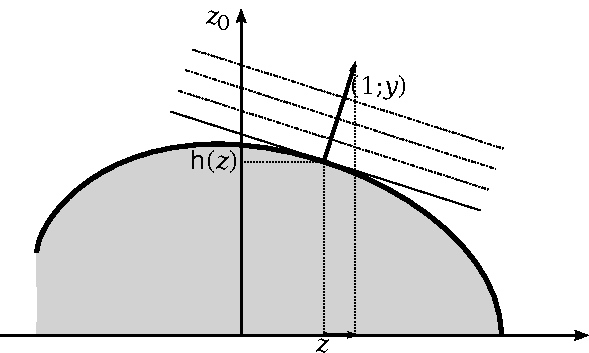
\includegraphics[scale=1]{diagramme1Da.pdf}
\caption{ An entropy-potential diagram $\cD$ represented in the $d=1$ case (beware: first coordinate $z_0$ represented by the \emph{vertical} axis): $\Pf(y)$ is obtained by sliding a line along the normal vector $(1; y)$ until it touches the hypograph of $\hf$, which happens above some $ z$ where $\grad \hf(z) = - y$. At this point $\grad \Pf(y)= z$: changing the direction $ y$ makes the touching line ``roll'' along the upper side of $\cD$; this rolling combines the rotation of $y$ and a normal translation given by scalar product with $z$.}\label{fig:diagramme1Da}
\end{figure}



\subsection{Set of nonlinear equilibrium measures}

%\newcommand\LEM{\mathscr{LEM}}

We now identify the fully nonlinear equilibrium measures, that is, the elements of $\EM(T,F,\vpot)$ (or just $\EM$) from Definition~\ref{def-fully-nonlin}. We define the set of \emph{$(G,\vpot)$-equilibrium values} to be
\[
\scV:=\left\{\mu(\vpot):\mu\in\EM\right\}.
\]

For $ z\in \rs(\vpot)$, recall the notations $\cM(z)$ and $\hf(z)$ from Definitions~\ref{defi-entropy}~and~\ref{defi-regular}. We start with Theorem~\ref{thm-equilibria}, in a version generalized to fully nonlinear pressures (see Definition~\ref{def-fully-nonlin}). We recall that $G$ is defined on some open set $V\subset \R\times \R^{d}$ and in the following $\partial_{i}G$ stands for $\partial G/\partial z_{i}$, $i=0,1,\,\ldots,\,d$.

\begin{theo}\label{thm:equilibria-G}
Let $(T, \pot)$ be a {$C^r$ Legendre system} for some $1\leq r\leq\omega$ and let $\Pi^G$ be a fully nonlinear pressure defined by an admissible $C^r$ function $G$.

Then the set $\EM$ of $(G,\vpot)$-equilibrium measures is a nonempty and compact set of linear equilibrium measures. More precisely,
\begin{enumerate}\romanenumi
\item\label{enumi:equilibria-G-i}
$\scV = \{ z\in\interior(\rs(\vpot)):G(\hf(z); z)\text{ maximal }\}$ is a nonempty compact set on which
\begin{equation}\label{eq-gradg}
0 = \grad G + \partial_{0} G \cdot \grad \hf \quad \text{where } \grad := \left(\partial_1,\,\dots,\,\partial_d\right).
\end{equation}
\item\label{enumi:equilibria-G-ii}
$ \EM$ is the set of all linear equilibrium measures with respect to all potentials $y\cdot\vec\pot$ where $y \in -\grad \hf(\scV)$.
\end{enumerate}
\end{theo}

\begin{proof}
We prove assertions~\eqref{enumi:equilibria-G-i} and~\eqref{enumi:equilibria-G-ii}, the rest being immediate consequences.

Let us note that a measure $\mu\in\Prob(T)$ is a fully nonlinear equilibrium measure if and only if
\[
G(h(T,\mu);\mu(\vpot)) = \sup_{(z_0; z)\,\in\,\CD} G(z_0; z) = \sup_{z\,\in\,\rs(\vpot)} g(z) \text{ where }g(z):=G(\hf(z); z).
\]
Indeed, the first equality follows from the definitions and the second one follows from the fact that $z_0\mapsto G(z_0; z)$ is increasing for each $ z\in\rs(\vpot)$. Since $g$ is continuous on the compact set $\rs(\vpot)$, it follows that $\scV$ is itself compact provided the maximum is not achieved on the boundary. This follows from the next:

\begin{claim}\label{claim-boundary}
Since $h$ is concave with $\lvert \grad\hf \rvert\to\infty$ at the boundary of $\rs(\vpot)$, we have $\scV\subset\inter(\rs(\vpot))$.
\end{claim}

\begin{proof}[Proof of the claim]
Consider a point $z_0$ on the boundary of $\rs(\vpot)$, and let us prove that it cannot maximize $g$. Let $\vec u$ be any vector such that $z_0+\vec u\in\inter(\rs(\vpot))$; by convexity of $\rs(\vpot)$, for all $t\in(0,1]$ we also have $z_0+t\vec u\in\inter(\rs(\vpot))$ and we define $f(t) = \hf(z_0+t\vec u)$. By concavity the derivative of $f$ has a limit, finite or infinite, as $t\to0$. For all {small enough} $t>0$, we have $f'(t) = \grad\hf(z_0+t\vec u) \cdot \vec u$. We know that $\lvert\grad \hf\rvert\to\infty$ at the boundary, but it could {\it a priori} be that $\grad \hf$ becomes orthogonal to $\vec u$ as $t\to0$; we now prove that this cannot be the case.

At each small enough $t>0$, the tangent space $H_t$ over $z_0+t\vec u$ to the upper boundary of $\cD$ has $(1,-\grad\hf)$ as normal vector. As $t\to0$, $\lvert \grad\hf\rvert\to\infty$ so that any accumulation point $H_0$ of $H_t$ is vertical, of the form $\RR\times L$ where $L$ is a hyperplane of $\RR^d$ (normal to an accumulation point of the direction of $\grad\hf(z_0+t\vec u)$). Since $\cD$ is contained in a half-space delimited by $H_0$, $L$ must be a supporting hyperplane of $\rs(\vpot)$ at $z_0$. Since $\vec u$ has been chosen pointing to the interior of $\rs(\vpot)$, the angle between $\vec u$ and $L$ is bounded away from $0$. It follows that for some constant $c>0$ and all $t>0$, $\grad\hf(z_0+t\vec u)\cdot\vec u \ge c\lvert \grad\hf(z_0+t\vec u)\rvert \lvert \vec u\rvert\to\infty$.

We deduce that $f'(t)\to+\infty$ as $t\to0$. Since $\partial_0G>0$, it is bounded away from $0$ on the segment with endpoints $z_0$ and $z_0+\vec u$ and it follows that $g(z_0+t \vec u)-g(z_0)\gg t$ as $t\to0$. In particular there exists $t>0$ such that $g(z_0+t \vec u)>g(z_0)$.
\end{proof}


It follows that $\grad g = 0$ on $\scV$. Now,
\begin{equation}\label{eq-grad-g}
\grad g = \grad G + \frac{\partial G}{\partial z_0} \grad \hf.
\end{equation}
Eq.~\eqref{eq-gradg} follows and assertion~\eqref{enumi:equilibria-G-i} is established.

Let $\nu\in\EM$. The above remarks show that $\nu$ maximizes the entropy in $\cM(z)$ where $ z:=\nu(\vpot)$. By Proposition~\ref{prop:nlem}, this implies that $\nu$ is an equilibrium measure for $y\cdot\vpot$ where $ y:=-\grad\hf(z)$, yielding the inclusion
\[
\EM \subset \left\{ \nu \text{ equilibrium measure for }y\cdot\vpot : y\in -\grad\hf(\scV)\right\}.
\]
To check the converse inclusion, let $ z\in\scV$ and apply Proposition~\ref{prop:nlem}. Setting $y:=-\grad\hf(z)$ and taking $\nu_y$ to be an equilibrium measure for $y\cdot\vpot$ we get $ z:=\grad\Pf(y)$ and $G(h(T,\nu_{ y});\nu_{ y}(\vpot))=g(z)$ which is maximum since $ z\in\scV$. Hence $\nu_{ y}\in\EM$. Assertion~\eqref{enumi:equilibria-G-ii} is established.
\end{proof}


\begin{rema}
The value $\max_{\Prob(T)} \FNLP$ is a generalization of our previous definition of nonlinear pressure. Of course, one could decide to study the variational principle for full general $G$ without any restriction. Nevertheless we point out that:
\begin{itemize}
\item[\eqref{enumi:equilibria-G-i}] Assumption $\inf\partial_0 G>0$ is crucial: a change of sign would modify the nature of the problem,
\item[\eqref{enumi:equilibria-G-ii}] the case $G(z_0; z) = z_0+F(z)$ is of particular interest: in the classical variational principle, the term $h(T,\mu)$ comes from the summation over $(\eps,n)$-covers in the Gibbs measures (see Formula~\eqref{eq:NLP}), and there is at the moment no candidate to replace this summation and define a \emph{topological} pressure in the case of a general $G$.
\end{itemize}
\end{rema}

\begin{rema}\label{rem-max-ent-cond}
The proof of Theorem~\ref{thm:equilibria-G} contains the following variation on~\cite[Theorem~B]{KW2015} and~\cite[Theorem~G]{GKLM}: if $(T,\vec\pot)$ is a $C^1$ Legendre system and if $\mu_{0}\in\Prob(T)$ maximizes $h(\mu) { +\mu(\psi)}$ subject to $\mu(\vec\pot)=z$ for some $z\in\inter(\rs(\vec\pot))$, then $\mu_0$ is a linear equilibrium measure for some potential $\psi+y\cdot \vec\varphi$ where $y\in\RR^d$. This particular statement can be obtained as soon as $\lvert \grad \hf(x_i)\rvert\to\infty$ for all sequences $(x_i)$ of $\inter\rs(\vec \varphi)$ tending to the boundary, reasoning similarly to the proof of Proposition~\ref{prop-interior} and using Claim~\ref{claim-boundary}.
\end{rema}

\begin{rema}
We can also apply the same method to the mean field models of Section~\ref{subsubsec-mft}, with energy maps: $\En(\mu)=\int_X V(x,\mu(\vec\pot))\, d\mu(x)$ such that $V$ is Lipschitz. Indeed, Claim~\ref{claim-boundary} shows that if $\mu_0$ is a nonlinear equilibrium measure, then the condition $z_{\opt}:=\mu_{ 0}(\vec\pot)\in\inter\rs(\vec\pot)$ is satisfied. Setting $\psi(x):=V(x,z_{\opt})$, $\mu_0$ then also maximizes $h(T,\mu)+\mu(\psi)$ under the constraint $\mu(\vec \varphi)=z_{\opt}$, and must thus be a linear equilibrium measure for some $\psi+y\cdot \vec \varphi$.
\end{rema}

To state our next result, we recall that a \emph{subvariety} of an open set $W\subset\RR^d$ is a subset defined by finitely many functions $h_1,\,\dots,\,h_k\in C^r(W)$ as $\{x\in W: h_1(x)=\dots=h_k(x)\}$. If $r=\omega$, it is easy to see that any nontrivial subvariety has zero Lebesgue measure (see, e.g., \cite{Mityagin} for a simple proof).


The previous theorem implies the following, which in particular contains Theorem~\ref{thm-finiteness}.

\begin{coro}
Let $(T, \vpot)$ be a $C^\omega$ Legendre system and $G$ be a $C^\omega$ admissible function defined on an open set $V\subset \RR^{1+d}$. Then the set $\scV$ of $(G,\vpot)$-equilibrium values is a compact subset of an analytic sub-variety of $\RR^d$.

In particular, it is a closed set with empty interior which is Lebesgue negligible.
\end{coro}

Since a proper analytic sub-variety of a compact line segment is finite:

\begin{coro}\label{cor-finite-1D}
Let $(T,\pot)$ be a $C^\omega$ Legendre system with unique equilibrium measures and $G$ be a $C^\omega$ admissible function with $d=1$, then the set $\EM$ of equilibrium measures is finite.
\end{coro}

When $d\ge2$, we have a \emph{generic} uniqueness.

\begin{prop}\label{p-generic-unique}
Let $(T, \vpot)$ be a $C^r$ Legendre system with unique equilibrium measures for some $2\leq r\leq\omega$. There is a unique nonlinear equilibrium measure in both of the following settings:
\begin{enumerate}\romanenumi
\item\label{enumi:generic1}
For $G$ in some open and dense subset of $\{G\in C^r(V):\partial_0 G>0\}$ where $V$ is a given admissible open subset of $\RR\times\RR^d$;
\item\label{enumi:generic2}
For $G(z_0;z)=z_0+F(z)$ with $F$ in some open and dense subset of $C^r(U)$ where $U$ is a given open neighborhood of $\rs(\vpot)$ in $\RR^d$.
\end{enumerate}
\end{prop}

Claim~\eqref{enumi:generic2} above means that, for a generic nonlinearity $F$, there is a unique nonlinear equilibrium measure. It is not implied by the fully nonlinear case~\eqref{enumi:generic1} since the corresponding set of $G$s has empty interior. It would be interesting to determine conditions on a fixed non-linearity $F$ or $G$ under which a generic $\vpot$ leads to a unique equilibrium measure.

%\medbreak

In higher dimension $d\ge 2$, we do not know whether finiteness holds in the real-analytic case. For smooth functions, even finiteness may fail.


\begin{prop}\label{prop-flexibility}
Let $(T, \vpot)$ be a {$C^r$ Legendre system} for some $2\leq r\leq\infty$. For all compact sets $\emptyset\ne E\subset\interior \rs(\vpot)$, there exists a $C^r$ nonlinearity $F$ such that the set of equilibrium values $\scV$ equals $E$.

In particular the set of equilibrium measures can be infinite, even uncountable.
\end{prop}

One could rephrase the previous proposition in terms of the set $\scY$ since it is equal to $-\grad \hf(\scV)$ where $-\grad\hf:\RR^d\to\inter\rs(\vpot)$ is a diffeomorphism.

%\medbreak

Before proving these two propositions, we recall some well-known facts about Morse functions. Given any open subset $U\subset\RR^d$, a function $g\in C^r(U)$ with $2\leq r\leq\omega$ is Morse on $K\subset U$ if no critical point in $K$ is degenerate and it is nonresonant if it takes distinct values at each of its critical points in $K$~\cite[Definitions~1.1.7 and 1.2.11]{Nicolaescu}. In particular, it has at most one maximizer on $K$. Finally, the set of nonresonant Morse $C^r$ functions on a compact set is open and dense (see the proofs in~\cite[Section~1.2]{Nicolaescu}). This is to be understood with respect to the classical uniform topologies on $C^r(U)$ with finite $r$, or the limit topology for $C^\infty(U)$, or the more complicated standard topology of $C^\omega(U)$ (see, e.g., \cite[p.~53]{Krantz-Parks}).


\begin{proof}[Proof of Proposition~\ref{p-generic-unique}]
We prove Claim~\eqref{enumi:generic1}. The proof of Claim~\eqref{enumi:generic2} is entirely similar. Note that it is enough to prove the claim under the auxiliary assumptions $\partial_0 G>1/C$ and $\lvert \grad G\rvert < C$ for $C>0$ arbitrary.

First note that, by~\eqref{eq-grad-g}, $0=\grad g$ implies that $\lvert\grad \hf\rvert \leq C^2$. Hence, it is enough to ensure that $G$ is nonresonant Morse on the compact subset:
\[
K:=\left\{z\in V: \lvert\grad\hf\rvert\leq C^2\right\}.
\]
Second, observe that $G\mapsto g$ is continuous from $C^r(V)\to C^r(\interior\rs(\vpot))$. Therefore the set $\CG$ of $G\in C^r(V)$ such that $g$ is nonresonant and Morse on $K$ is open.

Third, given any $g\in C^r(V)$, the map $k\mapsto g+k$ is a self-homeomorphism of $C^r(V)$. Therefore there are arbitrarily small $k\in C^r(V)$ such that $g+k$ is nonresonant and Morse on $K$. Considering $\tilde G(z_0,\,\dots,\,z_d):=G(z_0,\,\dots,\,z_d)+k(z_1,\,\dots,\,z_d)$ shows that $\CG$ is dense in $C^r(V)$.
\end{proof}


\begin{proof}[Proof of Proposition~\ref{prop-flexibility}]
Let $f:\RR^d\to [0,\infty)$ be a $C^\infty$ function such that $E=\{ z\in\RR^d \mid f(z) = 0\}$ (such a function can be constructed as a convergent sum of functions that are each positive on one open balls, with the union of the balls equal to the complement of $E$). Let $F$ be $-1$ outside $\interior\rs(\vpot)$, coincide with $-f-\hf$ on a compact subset of $\interior\rs(\vpot)$ containing $E$ in its interior, and be less than $-\hf$ in between; such a function exists since $E$ does not approach the boundary of the rotation set. Then maximizing $\hf(z)+F(z)$ is the same as minimizing $f(z)$, i.e., making it vanish and is achieved precisely on $E\ne\emptyset$.
\end{proof}



\section{Examples of phase transitions}\label{sec-examples}

This section is devoted to the application of the framework developed above to a few families of systems whose energy depends on a real multiplicative parameter (i.e., an inverse temperature) and exhibiting various behaviors when this parameter is modified: changes in the number of equilibrium measures, piecewise analytic behavior with or without an affine piece. Most examples belong to the non-linear thermodynamical formalism, but even in the linear case we provide new insight thanks to the entropy-potential diagram $\cD$, see Theorem~\ref{thm-fpt-linear}.



\subsection{The Curie--Weiss Model -- Symmetric case}\label{sec-Curie-Weiss}

The \emph{Curie--Weiss energy} for a potential $\pot$ is given by a quadratic nonlinearity, i.e., $\En(\mu) = \beta\En_1(\mu) = \frac{1}{2} \beta \mu(\pot)^2$ where $\beta$ is a parameter called the \emph{inverse of temperature}. For this specific case, we shall first use our general machinery above to recover an example treated in~\cite{Leplaideur-Watbled}, then provide a second example exhibiting a ``metastable'' phase transition.

We consider here the left shift $T$ on $X:=\{a,b\}^\N$, endowed for example with the distance
\[
d(x,y)=2^{-\inf\{i\,\mid\,x_i\neq y_i\}} \qquad \text{where } x=(x_i)_{i\,\in\,\NN}, y=(y_i)_{i\,\in\,\NN},
\]
with the potential $\pot:X\to\RR$ defined by
\[
\pot(x)=
\begin{cases}
-1 &\text{if }x_0 = a \\
1 &\text{if }x_0 = b
\end{cases}
\]
and the Curie--Weiss nonlinearity $F(z) = \beta F_1(z):=\frac{1}{2}\beta z^{2}$, with $\beta\ge 0$.

For any given $z\in\rho(\varphi)=[-1,1]$, we consider the invariant measures $\mu\in\cM(z)$, i.e., such that $\mu([b])-\mu([a])=z$ where $[i]$ is the cylinder of words starting with the letter $i$. Since these two cylinders form a partition of $X$, this equation rewrites as $\mu([a]) =\frac{1-z}{2}$ (and therefore $\mu([b])=\frac{1+z}{2}$). Among invariant measures in $\cM(z)$, the one of maximal entropy is the Bernoulli measure with weights $(\frac{1-z}2,\frac{1+z}2)$, whose entropy is well-known:
\[
\hf(z) = -\frac{1-z}{2}\log\frac{1-z}{2} -\frac{1+z}{2}\log \frac{1+z}{2}.
\]
We thus are left with maximizing, given $\beta\ge 0$,
\[
P_\beta(z):= \hf(z)+ \beta F(z) =-\frac{1-z}2\log\frac{1-z}2-\frac{1+z}2\log\frac{1+z}2 + \frac12 \beta z^{2}.
\]
A simple computation shows that there are two cases (see Figure~\ref{fig:CurieWeiss}):
\begin{enumerate}\romanenumi
\item For $0\le \beta\le 1$, $0$ is the unique critical point of $P_\beta$ and is indeed a maximum. Thus, $\scV=\{0\}$, there is a unique equilibrium state which is the Bernoulli measure of weights $(\frac12,\frac12)$, and the nonlinear topological pressure is $\NLP^{\beta\En_1}_\top(T) = \log 2$.
\item For $\beta>1$, there are three distinct critical points $\{-z_\beta,0,z_\beta\}$ among which $0$ is a local minimum and $-z_B<z_B$ are two global maxima. Hence, $\scV=\{-z_\beta,z_\beta\}$ and there are two equilibrium measures, which are ``symmetrical'' Bernoulli measures, one with $\mu([a])=\frac{1-z_\beta}{2}$ the other with $\mu([b])=\frac{1-z_\beta}{2}$.
\end{enumerate}
We have recovered the result of~\cite{Leplaideur-Watbled} that the nonlinear equilibrium measure is unique for $0\leq \beta\leq 1$ but that there are two of them for $\beta>1$, in line with the physical model.

\begin{figure}
\centering
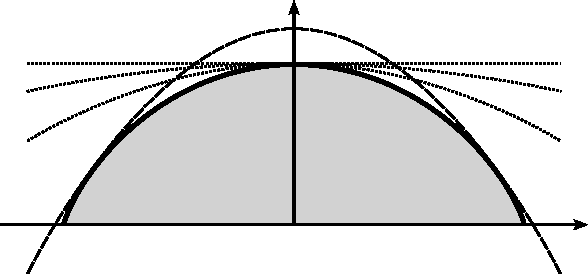
\includegraphics[scale=1]{CurieWeiss.pdf}
\caption{The symmetric Curie--Weiss example: graph of $\hf$ (solid line), highest translates of the graph of $-\beta F$ touching it (dotted lines: $\beta<1$; dashed line: $\beta>1$).}\label{fig:CurieWeiss}
\end{figure}

Note that any $C^2$ Legendre system $(T,\pot)$ with an entropy-potential diagram that is symmetric with respect to the vertical axis will provide a similar example. Indeed the symmetry ensures that for all $\beta$, $0$ is a critical point; and as long as $\beta<\hf''(0)$, the graph of $\hf$ being more concave at $0$ than the graph of $-\beta F$, $0$ will be a local maximum. It will then be a global maximum at least when $\beta$ is close enough to $0$. For $\beta>\hf''(0)$, $0$ will be a local minimum and one will get (at least) two non-zero symmetric equilibrium values.



\subsection{An asymmetric Curie--Weiss model}\label{sec-metastable}

Consider now the space of three-letter words $X=\{a,b,c\}^{\NN}$ and let $T$ be the left shift on $X$. We will again consider the Curie--Weiss nonlinearities $F(z) = \beta F_1(z) = \beta\frac{z^2}{2}$ where $\beta\in[0,+\infty)$ is the inverse of the temperature, but with a potential exhibiting a specific asymmetry:
\[
\pot(x) =
\begin{cases}
-2 &\text{when }x_0=a \text{ or }x_0=b,\\
3 &\text{when }x_0=c.
\end{cases}
\]
Here $\rho(\pot)=[-2,3]$ and a measure maximizing entropy under the constraint $\mu(\pot)=z$ must, as above, be a Bernoulli measure. If we write $(p,q,1-(p+q))$ for its weights, the constraint translates as
\begin{equation}
p+q = \frac{3-z}{5}.
\end{equation}
Given this constraint, it is easily checked that entropy is maximized when $p=q$. Setting $p(z) = (3-z)/10$, we get that the measure in $\cM(z)$ maximizing entropy is the Bernoulli measure with weights $(p(z),p(z),1-2p(z))$ and we obtain
\begin{align*}
\hf(z) &= -2p(z)\log p(z)-(1-2p(z))\log(1-2p(z)) \\
&= \frac{z-3}{5} \log\frac{3-z}{10}-\frac{2+z}{5}\log \frac{2+z}{5}.
\end{align*}
We are left with maximizing
\[
P_\beta(z) := \hf(z)+\beta F_1(z) = \frac{z-3}{5} \log\frac{3-z}{10}-\frac{2+z}{5}\log \frac{2+z}{5} +\frac12\beta z^2
\]
for $z\in[-2,3]$. The critical points of $P_\beta$ are given by the intersections of the graph of $\hf'$ with the line $\ell_\beta=\{(z_0,z)\mid z_0=-\beta z\}$. We have
\begin{align*}
\hf'(z) &= \frac{1}{5} \log\left(\frac{3-z}{4+2z} \right) \\
\hf''(z) &= -\frac{1}{(2+z)(3-z)} = \frac15\left(\frac{1}{z-3} -\frac{1}{z+2} \right) \\
\hf'''(z) &= \frac15\left(\frac{1}{(z+2)^2} -\frac{1}{(z-3)^2} \right)
\end{align*}
so that $\hf'$ is strictly decreasing, from $+\infty$ when $z\to-2$ to $-\infty$ when $z\to 3$; it has a single inflection point at $z=\frac12$, is convex on $(-2,\frac12]$ and concave on $[\frac12,3)$ (see its graph in Figure~\ref{fig:hprime}).

It follows that for $\beta\ge 0$ small enough, $P_\beta$ has only one critical point, which must be a maximum; in this regime, there is only one equilibrium state, with equilibrium value $z<0$, and the pressure varies analytically.

\begin{figure}
\centering
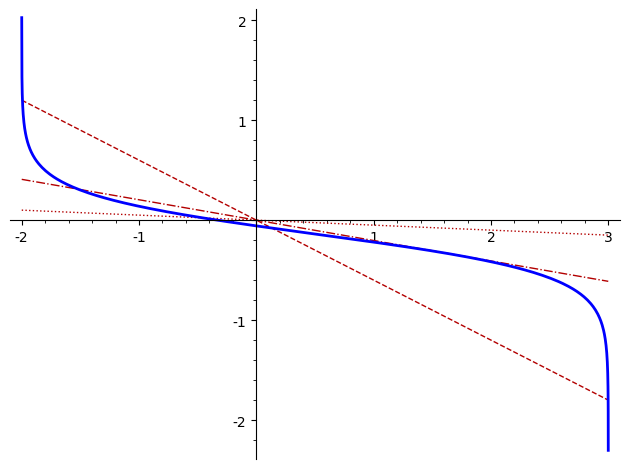
\includegraphics[width=.8\linewidth]{hprime.png}
\caption{The graph of $\hf'$ and $\ell_\beta$ for three values of $\beta$: $\beta<\beta_1$ (dotted), $\beta=\beta_1$ (dot dash), $\beta>\beta_1$ (dashed).}\label{fig:hprime}
\end{figure}

Increasing $\beta$, at some value $\beta_1$ the line $\ell_\beta$ touches the graph of $\hf'$ on the right, and a second critical point appears. However, at this moment there is still only one equilibrium measure: $P_\beta$ is unimodal, decreasing around the second critical point. Increasing $\beta$ any further makes $P_\beta$ bimodal, with three critical points: one local minimum located between two local maximums $z_1(\beta)<z_2(\beta)$.

At first, $z_1(\beta)$ is the unique global maximum, but it ultimately gets surpassed by $P_\beta(z_2(\beta))$, precisely at the inverse temperature $\beta_0$ when the vertical translate of the graph of $-\frac{\beta}{2} z^2$ touching the graph of $\hf$ does so at two points. The choice of $\pot$ has been made to ensure this happens, by giving the entropy-potential diagram a larger overhang to the right than to the left (see Figure~\ref{fig:metastable}): as $\beta\to\infty$, the highest translate of the graph of $-\beta F$ that touches the graph of $\hf$ converges to the two vertical lines of equations $(z=3)$ and $(z=-3)$. The latter of these vertical lines is far from the entropy-potential diagram since $\rs(\pot)=[-2,3]$, and for large enough $\beta$ the unique global maximum of $P_\beta$ must be attained at $z_2(\beta)\to 3$.

\begin{figure}
\centering
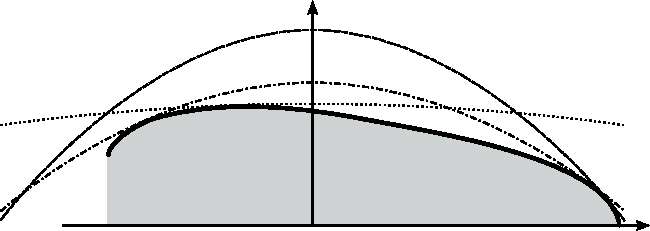
\includegraphics[scale=1]{metastable.pdf}
\caption{A metastable phase transition: graph of $\hf$ (solid line, graph modified for readability), highest translates of the graph of $-\beta F_1$ touching it (dotted: $\beta<\beta_0$; dashed: $\beta>\beta_0$; dot-dashed: $\beta=\beta_0$).}\label{fig:metastable}
\end{figure}

Again the pressure is analytic for $\beta>\beta_0$, but we have a phase transition at $\beta_0$: the pressure is $\beta\mapsto \max(P_\beta(z_1(\beta)),P_\beta(z_2(\beta)))$ and cannot be analytical at the point where the arguments of the max cross each other. Observe that the value $\beta_1$ ($<\beta_0$) does not correspond to a phase transition: pressure is analytic in the vicinity of $\beta_1$.

This example motivates the following definition.


\begin{defi}
A system $(T,\En_1)$ is said to exhibit a \emph{metastable phase transition} at inverse temperature $\beta_0>0$ when there are two curves of invariant probability measures $(\mu_\beta)$, $(\nu_\beta)$ defined on a neighborhood $I$ of $\beta_0$ with $\beta\mapsto \NLP^{\beta\En_1}(\mu_\beta)$ and $\beta \mapsto \NLP^{\beta\En_1}(\nu_\beta)$ both $C^\omega$, such that:
\begin{enumerate}\romanenumi
\item for all $\beta\in I$, $(\mu_\beta)$, $(\nu_\beta)$ are local maximums of $\NLP^{\beta\En}$,
\item for $\beta<\beta_0$, $\mu_\beta$ is an equilibrium measure of $\beta\En$ but $\nu_\beta$ is not, and for $\beta>\beta_0$, $\nu_\beta$ is an equilibrium measure but $\mu_\beta$ is not.
\end{enumerate}
\end{defi}

Observe that the pressure function $\beta\mapsto \NLP^{\beta\En_1}$ is not analytic at $\beta_0$, for otherwise $\NLP^{\beta\En_1}(\mu_\beta)$ and $\NLP^{\beta\En_1}(\nu_\beta)$ would have to coincide and both $\nu_\beta$ and $\mu_\beta$ would be equilibrium measures throughout $I$.

The ``metastable'' terminology is suggested by the analogy with the physical phenomenon of the same name. A simple example of it is that of water remaining liquid below the freezing point in some circumstances. This is modeled by the liquid state (described by $\mu_\beta$) admitting a continuation to $\beta>\beta_0$ as a local maximum and the global maximal, the solid state (described by $\nu_\beta$), being too far from $\mu_\beta$ to allow the water to easily reorganize itself from one state to the other. 


What we have proven can be summarized as follows.

\begin{theol}\label{th-metastable}
There exists a locally constant potential $\pot$ on a full shift $X$ such that the Curie-Weiss energy $\En_1(\mu) = \frac12 \mu(\pot)^2$ exhibits a metastable phase transition.
\end{theol}

This gives another concrete example of multiple nonlinear equilibrium measures in a context where the linear thermodynamical formalism is long known to be flawless (analytic pressure, etc.)



\subsection{The mean-field Potts model}\label{subsec:potts}

The mean-field Potts model is given by the full shift $(X,T)$ over a finite alphabet $\{\theta_{1},\,\ldots,\,\theta_{n}\}^{\N}$ or $\{\theta_{1},\,\ldots,\,\theta_{n}\}^{\Z}$, with $n\geq3$. The potential is $\vec\pot:=(\mathbbm{1}_{\theta_{1}},\,\ldots,\,\mathbbm{1}_{\theta_{n}})$ and the nonlinearity $F(z)=\beta F_1(z)=\frac\beta2 \lvert \vec z\rvert^2$ where $\lvert\cdot\rvert$ is the usual Euclidean norm. The energy is thus given by
\[
\En(\mu) = \beta\En_1(\mu)=\frac\beta2 \left\lvert\int \vec\pot \dd\mu\right\rvert^2 = \frac\beta2 \sum_i \mu([\theta_i])^2
\]
where, as above, $[\theta_i]$ is a cylinder, the set of words having the letter $\theta_i$ in zeroth position.

The framework developed above seems not to apply since the potentials are not linearly independent up to (coboundaries and) constants: $\sum_i \mathbbm{1}_{\theta_{i}} \equiv 1$, and the rotation set has empty interior. Let us take this as an opportunity to explain how this hypothesis is easily recovered: one simply extracts a maximal independent subfamily of potentials, here $\vec\pot_\circ = (\mathbbm{1}_{\theta_{1}},\ldots, \mathbbm{1}_{\theta_{n-1}})$, and adjusts the nonlinearity to ensure $F_\circ(\mu(\vec\pot_\circ))=F(\mu(\vec\pot))$ for all $\mu\in\Prob(T)$, here
\[
F_\circ(z_1,\,\dots,\,z_{n-1}) = \frac\beta2 \left(z_1^2+\dots+z_{n-1}^2+\left(1-\sum_{i\,<\,n} z_i\right)^2\right).
\]
It is always possible to construct such an $F_\circ$, since by maximality each the potentials that are present in $\vec \pot$ can be expressed as linear combination of the potentials in $\vec\pot_\circ$ up to a coboundary and a constant, and a coboundary $g-g\circ T$ can be neglected since $\mu(g-g\circ T)=0$ for all invariant measures $\mu$.

Now $(T,\vec\pot_\circ)$ is {$C^\omega$ Legendre} and we can apply Theorems~\ref{thm-existence-NL} and~\ref{thm-equilibria} (recall that moreover $(T,\vec\pot_\circ)$ has unique linear equilibrium measures, hence each $z\in\scV$ yields a unique nonlinear equilibrium measure), and these results translate to the original system $(T,\vec\pot)$ with the nonlinearity $F$: accumulation points of Gibbs ensembles are convex combinations of the nonlinear equilibrium measures, each of which coincides with a linear equilibrium measure for some linear combination of the $(\pot_i)$; however, due to the lack of independence, several different linear combinations lead to the same equilibrium state.

In the specific case of the mean-field Potts model one can work out the equilibrium measures by (nontrivial) direct computations. Given a vector $z:=(z_{1},\,\ldots,\,z_{n})$ in the rotation set
\[
\rs(\vec\pot) :=\left\{\int\vec\pot\,d\mu,\ \mu\in\Prob(T)\right\} = \left\{(z_1,\,\dots z_n) \in [0,1]^n \colon \sum_i z_i = 1\right\},
\]
the maximal entropy among invariant measures $\mu$ satisfying $\mu(\vec\pot)=z$ is $\hf(z)=-\sum_{i}z_{i}\log z_{i}$ with the convention $0\log 0=0$. It is achieved by a unique measure, the Bernoulli measure giving each cylinder $[\theta_i]$ the mass $z_i$.

For $\be\ge 0$, the nonlinear pressure is
\[
\NLP_\top^{\beta\En_1}=\max_{\vec z}-\sum_{i}z_{i}\log z_{i}+\frac{\be}{2}\sum_{i}z_{i}^{2}.
\]


We now summarize results from~\cite{EllisWang90}. For $0 \le \be<\be_{c}:= 2\frac{n-1}{n-2}\log(n-1)$, $\NLP_{\top}^{\beta\En_1}$ is reached for $z=(\frac1n,\,\dots,\,\frac1n)$. The value is $\frac\be{2n}+\log n$ and is achieved by a unique measure.

For $\be>\be_{c}$, $\NLP_{\top}^{ \beta\En_1}$ is given by an implicit equation. It is realized by $z$ equal to any permutation of $\widetilde{z}$ defined by
\[
\widetilde{z}_{1}=\frac{1+(n-1)s}n,\ \widetilde{z}_{i}=\frac{1-s}n,\ 2\le i\le n
\]
where $s$ is the biggest solution for
\[
s=\frac{1-e^{-\be s}}{1+(n-1)e^{-\be s}}.
\]
Each permutation of $\widetilde{z}$ gives a distinct equilibrium measure. Thus we get exactly $n$ equilibrium measures.

For $\be=\be_{c}$, the maximal value is simultaneously realized by ($\frac1n,\,\ldots,\,\frac1n)$ and by the $n$ distinct permutations of $\tilde z$. Thus we get exactly $n+1$ equilibrium measures. In this case, the convergence of Gibbs measures to a convex combination of these equilibrium measures was previously shown in~\cite{Leplaideur-Watbled-2}.



\subsection{Freezing phase transitions}\label{sec:transition}

Let us explain how the entropy-potential diagram can be used to visualize ``freezing phase transitions'', i.e., situations where for some $\beta_0$, the set of equilibrium measures of the energy $\beta\En_1$ is constant for $\beta>\beta_0$. These measures are called the \emph{ground states}. The physical interpretation is that once the temperature goes below some positive value $1/\beta_0$, the system freezes in a macroscopic state corresponding to zero temperature, described by (one of) the ground states. In the linear thermodynamical formalism, the first freezing phase transition was exhibited by Hofbauer~\cite{Hofbauer}, motivated by giving examples with multiple equilibrium states (this is sometimes achieved at $\beta=\beta_0$). Concretely, the typical examples are the shift $T$ on $X = \{a,b\}^\NN$ or $X = \{a,b\}^\ZZ$ with potentials
\[
\pot(x) = -\frac{1}{k(x)^\alpha}, \qquad k(x) := \min\{\lvert k\rvert \colon x_k\neq a\}
\]
with $\alpha\in(0,1]$, and the freezing equilibrium measure is $\mu_0=\delta_{aaa\dots}$. It has more recently been shown by Bruin and Leplaideur~\cite{Bruin-Leplaideur1, Bruin-Leplaideur2} that one can produce in a similar way a freezing phase transition with more interesting ground states, supported on some uniquely ergodic, zero-entropy compact subsets of $X$ such as given by the Thue--Morse or the Fibonacci substitutions.

Let us interpret in the entropy-potential diagram $\cD$ such a freezing phase transition, with potential $\pot$ being maximized by some invariant measure $\mu_0$, say with $\mu_0(\pot)=0$ for normalization. By definition, for $\beta\ge\beta_0$ the pressure is affine and achieved at $\mu_0$, meaning that all lines of slope $<-\beta_0$ touching $\cD$ do it at the same point (see Figure~\ref{fig:freezing}).

\begin{figure}
\centering
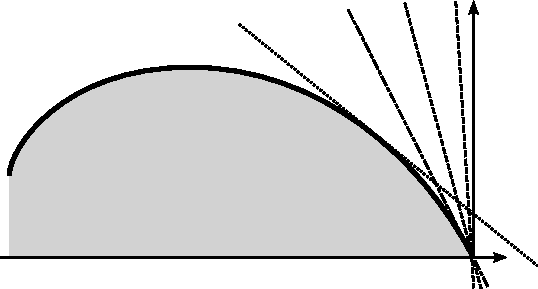
\includegraphics[width=.48\linewidth]{freezing.pdf}
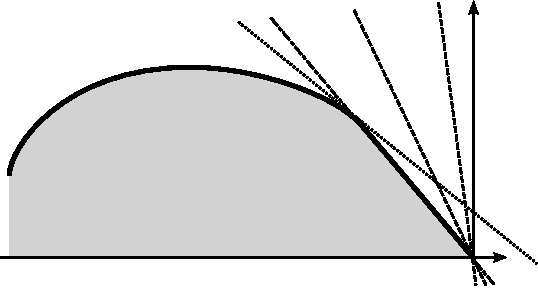
\includegraphics[width=.48\linewidth]{freezing2.pdf}
\caption{Freezing phase transitions in the linear thermodynamical formalism: for $\beta>\beta_0$, all support lines are concurrent, and $\cD$ must exhibit an acute corner at its right end. Left: $\hf$ is strictly concave, there might be a unique equilibrium measure throughout (case $\alpha=1$ in Hofbauer's example). Right: $\hf$ has a flat part, at $\beta_0$ there are (at least) two ergodic equilibrium measure, one at each end of the flat edge (case $\alpha<1$ in Hofbauer's example).}\label{fig:freezing}
\end{figure}

This observation immediately implies a characterization of (linear) freezing phase transition by a linear inequality between the entropy and the integral of the potential.

\begin{prop}\label{prop-fpt}
Let $T:X\to X$ be a measurable map, $\pot:X\to\RR$ be a potential whose rotation set has the form $[r,0]$ for some $r\in(-\infty,0)$, such that there is an invariant measure $\mu_0$ realizing $\mu_0(\pot) = 0$ and maximizing entropy among such measures: $h(T,\mu_0)=\max \{h(T,\mu) \colon \mu\in \Prob(T), \mu(\pot)=0\}$. The following are equivalent:
\begin{enumerate}\romanenumi
\item\label{enumi:fpt1}
the linear thermodynamical formalism for the system $(T,\pot)$ exhibits a freezing phase transition, i.e., for some $\beta_0>0$ and all $\beta>\beta_0$, the set of equilibrium measures is non-empty and independent of $\beta$,
\item\label{enumi:fpt2}
there is some finite $\beta$ such that $\mu_0$ is an equilibrium measure for $\beta\pot$,
\item\label{enumi:fpt3}
the topological pressure function
\begin{align*}
\Pf \colon \RR &\to \RR \\
\beta &\mapsto \sup \{ h(T,\mu) + \beta\mu(\pot) \colon \mu\in\Prob(T) \}
\end{align*}
is affine on some interval $[\beta_0,+\infty)$,
\item\label{enumi:fpt4}
there exists $C>0$ such that $h(T,\mu) \le h(T,\mu_0) -C \mu(\pot)$ for all $\mu\in\Prob(T)$.
\end{enumerate}
When these conditions are realized, the critical inverse temperature, i.e., the least possible value of $\beta_0$, is the least possible $C$ in the entropy-potential inequality~\eqref{enumi:fpt4}. The intercept of the affine part of the graph of $\Pf$ is then the entropy of equilibrium measures after the freezing phase transition, and its slope is their energy $\mu(\pot)$ (here $0$ is given by the chosen normalization of the rotation set).
\end{prop}

\begin{proof}
The main novelty here is the observation that~\eqref{enumi:fpt4} characterizes Freezing Phase Transitions, but for the sake of completeness we prove all the equivalences, through the cycle \eqref{enumi:fpt1}$\implies $\eqref{enumi:fpt3}$\implies$ \eqref{enumi:fpt4}$\implies$\eqref{enumi:fpt2}$\implies$\eqref{enumi:fpt1}.

Assume \eqref{enumi:fpt1} and let $\mu_1$ be any equilibrium measure for any $\beta>\beta_0$. For all $\beta>\beta_0$ we get $\Pf(\beta) = h(T,\mu_1)+\beta\mu_1(\pot)$, an affine expression.

Convex duality translates angular points to flat regions and vice-versa; that $\Pf$ is affine on an interval means that the entropy-potential diagram has an angular point with a supporting line of slope $-\beta$ for each $\beta$ in the interval. Let us explain this, a simple case of what we left hidden behind the appeal to Legendre duality above. Using the notation $\hf(z)=\sup\{h(T,\mu) \colon \mu(\pot)=z\}$ for all $z\in[r,0]$, $\hf$ is concave thus continuous on $(r,0)$, and has a continuous extension $\bar\hf$ on $[r,0]$. We can the rewrite $\Pf(\beta)=\max_z \bar\hf(z)+\beta z$. Denoting by $z_\beta$ an abscissa realizing $\Pf(\beta)$, observe that for all $\eps>0$, $\Pf(\beta+\eps)\ge \bar\hf(z_\beta)+(\beta+\eps) z_\beta\ge \Pf(\beta)+\eps z_\beta$ so that the right derivative of $\Pf$ is at least $z_\beta$. Similarly, $\Pf(\beta-\eps)\ge \Pf(\beta)-\eps z_\beta$ shows that the left derivative is at most $z_\beta$. Whenever $\Pf$ is differentiable, $\Pf'(\beta)=z_\beta$. On an affine part, the derivative exists and is constant, therefore $z_\beta$ is (locally) constant and $\hf$ has an angular point. Moreover the abscissa of the angular point is the slope of the line extending the affine part of the graph of $\Pf$, while the ordinate of that point is the intercept of that line.

Item~\eqref{enumi:fpt3} thus implies that the entropy-potential diagram has an angular point with supporting lines of slope $-\beta$ for all $\beta\ge\beta_0$. Since slopes are arbitrarily high in magnitude, the abscissa of this angular point must be the supremum of the rotation set, i.e., $0$. It must then have ordinate equal to the supremum of the realizable entropies for this energy, i.e., $h(T,\mu_0)$. In particular, the entropy-potential diagram is constrained under a line of equation $(h(T,\mu)=h(T,\mu_0)-\beta_0 \mu(\pot))$, which is~\eqref{enumi:fpt4}.

Assume~\eqref{enumi:fpt4} and take any $\beta\ge C$. For all $\mu\in\Prob(T)$,
\[
h(T,\mu)+\beta\mu(\pot) \le h(T,\mu_0) + (\beta-C) \mu(\pot) \le h(T,\mu_0) = h(T,\mu_0)+\beta\mu_0(\pot)
\]
so that $\mu_0$ is an equilibrium measure for such $\beta$, proving~\eqref{enumi:fpt2}.

Assume~\eqref{enumi:fpt2}, let $\beta_1$ be such that $\mu_0$ is an equilibrium measure for $\beta_1\pot$ and $\beta>\beta_1$. For all $\mu\in\Prob(T)$, since $\mu(\pot)\le 0$ and $\mu_0(\pot)=0$,
\[
h(T,\mu)+\beta\mu(\pot) \le h(T,\mu)+\beta_1\mu(\pot) \le h(T,\mu_0)+\beta_1\mu_0(\pot) = h(T,\mu_0)+\beta\mu_0(\pot)
\]
and $\mu_0$ is an equilibrium measure for $\beta\pot$. It follows that the set of $\beta$'s such $\mu_0$ is an equilibrium measure for $\beta\pot$ is an interval $\beta_0,+\infty)$. The above computation shows that for all $\beta>\beta_0$, the set of equilibrium measure is $\{\mu\in\Prob(T) \colon \mu(\pot)=0, h(T,\mu)=h(T,\mu_0) \}$, and is thus independent of $\beta$.
\end{proof}

\begin{rema}
If we consider several potentials $\pot_1,\,\dots,\,\pot_d$, the condition in Legendre regularity that $\lvert\grad \hf\rvert$ goes to $+\infty$ as one approaches the boundary is violated exactly when some linear combination of the $(\pot_k)$ exhibit a (linear) freezing phase transition.
\end{rema}

The entropy-potential diagram makes it {clear} how to prove existence of freezing phase transition in both the linear and nonlinear settings. We divide Theorem~\ref{thm-fpt} of the introduction into two parts.

\begin{theo}\label{thm-fpt-linear}
Let $T:X\to X$ be a continuous map of finite, positive topological entropy such that $\mu\mapsto h(T,\mu)$ is upper semi-continuous. Consider $\mu_0\in\Prob_\erg(T)$ with zero entropy. Then there exists a continuous potential $\pot:X\to \RR$ such that the linear thermodynamical formalism of $(T,\pot)$ exhibits a freezing phase transition with ground state $\mu_0$. Moreover we can ensure that $\mu_0$ is the unique ground state, and that at the critical inverse temperature $\beta_0$ there are exactly two equilibrium states.
\end{theo}

In particular, if $K$ is a compact $T$-invariant {set} with zero topological entropy, then we can find a potential exhibiting a freezing phase transition supported on $K$. This broadly extends~\cite{Bruin-Leplaideur1, Bruin-Leplaideur2} by proving existence of freezing phase transitions for all zero-entropy subshifts, instead of very specific ones; but it is not constructive, since the potential $\pot$ is ultimately obtained through the Hahn-Banach theorem.

\begin{proof}
According to a Theorem of Jenkinson~\cite{Jenkinson}, there exists a continuous potential $\tilde\pot:X\to\RR$ such that $\mu_0$ is the unique equilibrium state of $\tilde\pot$, i.e., the unique maximizer of $h(T,\mu)+\beta\mu(\tilde\pot)$ for $\beta=1$. Since $h(T,\mu_0)=0$ is minimal, $\mu_0$ must be a maximizing measure for $\tilde\pot$. The conclusion then follows from Proposition~\ref{prop-fpt} applied to the adjusted potential $\pot=\tilde\pot-\mu_0(\tilde\pot)$.

To have a second equilibrium state at the critical inverse temperature, it suffices to consider an arbitrary ergodic measure $\mu_1$ of positive entropy: Jenkinson's theorem provides a continuous potential whose only ergodic equilibrium states (at $\beta=1$) are $\mu_0$ and $\mu_1$. This also fixes the critical inverse temperature at $\beta_0=1$.
\end{proof}

\begin{theo}\label{thm-fpt-nonlinear}
Let $T:X\to X$ be a continuous dynamical system of finite, positive topological entropy such that $\mu\mapsto h(T,\mu)$ is upper semi-continuous. Let $\pot:X\to(-\infty,0]$ be a continuous potential such that $K=\pot^{-1}(0)$ is $T$-invariant and has zero topological entropy.

Then there exists a continuous nonlinearity $F_1 : (-\infty,0]\to (-\infty,0]$ with $F(0)=0$ such that the energy $\En_1(\mu) = F_1(\mu(\pot))$ exhibits a ``strong freezing phase transition'' in the following sense. There is a $\beta_0>0$ such that:
\begin{itemize}
\item for each $\beta<\beta_0$ the energy $\beta \En_1$ has at least one equilibrium measure, and none of them are supported on $K$,
\item at $\beta=\beta_0$ there are several equilibrium measures, at least one supported on $K$ and one not supported on $K$,
\item for each $\beta>\beta_0$ the equilibrium measures are exactly the $K$-supported, $T$-invariant measures and the topological pressure function $\beta\mapsto \NLP^{\beta\En_1}_\top(T)$ is affine.
\end{itemize}
\end{theo}

Observe that here $F_1$ will only be continuous at $0$; we can extend it continuously to $\RR$, but we cannot make $F_1$ differentiable in a neighborhood of $0$.

\begin{proof}
Take for $F_1$ any increasing convex continuous function $(-\infty,0]\to(-\infty,0]$ such that $\hf(z) = o(-F_1(z))$ as $z\to 0$. Theorem~\ref{thm-var-prin-NL} ensures that equilibrium measures are found by optimizing $\hf(z)+\beta F_1(z)$ and then maximizing entropy in $\cM(z)$, as in Section~\ref{sec:convexity} (we did not assume Legendre regularity, but we assumed enough to ensure that each optimal $z$ comes with at least one equilibrium measure).

Since $\hf$ is bounded by $h_\top(T)$, for $\beta$ large enough the graph of $-\beta F_1$ is above the graph of $\hf$ except at $0$ where they meet. This means that for these $\be$s, $\hf(z)+\be F_1(z)$ is non positive and always negative for $z<0$, i.e., the unique optimal $z$ is $0$.

Let $\beta_0$ the least $\beta$ such that $\hf(z)\le -\beta F_1(z)$ for all $z$. Since $\hf(z) = o(-\beta_0 F_1(z))$ as $z\to 0$, there must be a touching point distinct from $0$, and we get two optimal values $z=0$ and $z=z_0<0$, and at least two equilibrium measures. For $\beta<\beta_0$, $z=0$ cannot be optimal anymore since $z_0$ is strictly better. The conclusion follows.
\end{proof}

A simple example can be worked out in the case of the shift over $X=\{a,b\}^{\NN}$ and the potential $\pot$ taking the values $0$ on the cylinder $[a]$ and $-1$ on the cylinder $[b]$. We have $\hf(z) \sim z\log(-z)$ at zero, so that we can take $F_1(z) = -(-z)^\alpha$ with any $\alpha\in(0,1)$: the nonlinear thermodynamical formalism associated with the energy
\[
\mu\mapsto -\lvert \mu(\pot)\rvert^\alpha
\]
exhibits a strong freezing phase transition with ground state $\mu_0=\delta_{aaa\dots}$.



\appendix
\section{Wasserstein energy}\label{sec-appendix}


We consider here the case of the doubling map $T:x\mapsto 2x\mod 1$ on the circle $X=\RR/\ZZ$ with energy $\En_1(\mu) = \wass_1(\mu,\lambda)$ where $\lambda$ is the Lebesgue measure and $\wass_1$ the Wasserstein distance of exponent $p=1$.

Consider the Bernoulli measures $(\mu_q)_{q\,\in\,[0,1]}$, defined as the unique fixed point of
\[
\mu\mapsto q S_*(\mu) + (1-q) R_*(\mu)
\]
where $S(x)=\frac12 x$ and $R(x)=\frac12 x+\frac12$; they interpolate between $\lambda=\mu_{\frac12}$ and $\delta_0=\mu_1$ ($=\delta_1=\mu_0$). To prove that for $\beta\in(0,+\infty)$ neither $\lambda$ not $\delta_0$ are equilibrium measures, the referee suggested to use the $\mu_q$ as contenders.

The entropy term of the nonlinear pressure is $h(T,\mu_q)=-q\log q-(1-q)\log(1-q)$ and has derivative $0$ at $q=\frac12$ and $-\infty$ at $q=1$; we are left with estimating the energy term $\wass_1(\mu_q,\lambda)$.

On the interval, the $1$-Wasserstein distance between $\mu_q$ and $\lambda$ would be exactly $\lvert q-\frac12\rvert$ (this can be obtained by monotone rearrangement, and is derived explicitly in~\cite{Fraser2015}). However this formula does not apply on the circle (e.g. $W_1(\lambda,\mu_1=\delta_0)=\frac14\neq\frac12$). Luckily, we can give a similar estimate.

\begin{lemm}
For all $q\in[0,1]$,
\[
\wass_1(\mu_q,\lambda)\le \left\lvert q-\frac12 \right\rvert
\]
and when $q\to 1/2$ from above,
\[
\wass_1(\mu_q,\lambda) \ge \frac18\left(q-\frac12\right)+o\left(q-\frac12\right).
\]
\end{lemm}

\begin{proof}
The upper bound follows from the aforementioned bound in the interval metric, since it is no lesser than the circle metric. To prove the lower bound we use Kantorovich duality (we actually only use the easiest part, namely that $\wass_1(\mu,\nu) \ge \lvert\int f \dd \mu -\int f \dd \nu\lvert$ for all $1$-Lipschitz $f$) with test function
\[
f(x) =
\begin{cases}
x &\text{when }x\in[0,1/4] \\
\frac12-x &\text{when }x\in[1/4,1/2] \\
0 & \text{when }x\in [1/2,1].
\end{cases}
\]
On the one hand $\int f \dd\lambda = \frac{1}{16}$; on the other hand we evaluate $\int f\dd\mu_q$ using the definition of $\mu_q$ given above:
\begin{align*}
\int f\dd\mu_q &= q\int f\circ S \dd\mu_q + (1-q) \int \underbrace{f\circ R}_{=0}\dd\mu_q \\
&= q^2\int f\circ S^2 \dd\mu_q(x) + q(1-q) \int f\circ S\circ R \dd\mu_q \\
&= \frac{q^2}{4} \int_0^1 x \dd\mu_q(x) + \frac{q(1-q)}{4} \int_0^1 (1-x) \dd\mu_q(x) \\
&= \frac{2q^2-q}{4}\int_0^1 x\dd\mu_q(x) + \frac{q(1-q)}{4}.
\end{align*}
We use the same trick to express $\int x\dd\mu_q(x)$ in term of itself:
\begin{align*}
\int_0^1 x \dd\mu_q(x) &= q\int_0^1 \frac12 x \dd\mu_q(x) + (1-q)\int_0^1\left(\frac12+\frac12x\right)\dd\mu_q(x) \\
&= \frac{1}{2}\int_0^1 x \dd\mu_q(x)+\frac{1-q}{2}\\
\int_0^1 x \dd\mu_q(x) &= 1-q,
\end{align*}
which plugged in the previous computation gives
\[
\int f\dd\mu_q = \frac{q^2(1-q)}{2}.
\]
It now suffices to use $\wass_1(\mu_q,\lambda)\ge\int f\dd\mu_q-\frac{1}{16}$ and the Taylor--Young formula:
\[
\frac{q^2(1-q)}{2} = \frac{1}{16}+\frac18\left(q-\frac12\right) + o\left(q-\frac12\right).
\]
\end{proof}

From the lower bound we deduce that for any $\beta>0$, the function $q\mapsto h(T,\mu_q) + \beta W_1(\lambda,\mu_q)$ has positive right upper derivative at $\frac12$ so that $\mu_{\frac12+\varepsilon}$ improves on $\lambda$ for small enough $\varepsilon$, and $\lambda$ cannot be an equilibrium measure. Similarly the upper bound shows that $q\mapsto h(T,\mu_q) + \beta W_1(\lambda,\mu_q)$ has derivative $-\infty$ at $q=1$, so that $\mu_{1-\varepsilon}$ improves on $\delta_0=\mu_1$ for any finite $\beta$.

Finally, observe that for $p>1$ Jensen's inequality yields $W_p(\mu_q,\lambda)>W_1(\mu_q,\lambda)$, and the same reasoning proves that $\lambda$ is not an equilibrium measure for any $\beta>0$.

\vspace*{10pt}


\begin{thebibliography}{99}
\bibitem{Baladi-book}Baladi, Viviane Positive transfer operators and decay of correlations, Advanced Series in Nonlinear Dynamics, 16, World Scientific, 2000 | Zbl | DOI
\bibitem{BarreiraHolanda2021}Barreira, Luis; Holanda, Carllos E. Higher-dimensional nonlinear thermodynamic formalism (2021) (https://arxiv.org/abs/2111.09853)
\bibitem{Brin-Katok}Brin, Michael; Katok, Anatole On Local Entropy, Geometric dynamics, Proc. int. Symp., Rio de Janeiro/Brasil 1981 (Lecture Notes in Mathematics), Volume 1007, Springer, 1983, pp. 30-38 | Zbl | MR
\bibitem{Bruin-Leplaideur1}Bruin, Henk; Leplaideur, Renaud Renormalization, thermodynamic formalism and quasi-crystals in subshifts, Commun. Math. Phys., Volume 321 (2013) no. 1, pp. 209-247 | Zbl | DOI | MR
\bibitem{Bruin-Leplaideur2}Bruin, Henk; Leplaideur, Renaud Renormalization, freezing phase transitions and Fibonacci quasicrystals, Ann. Sci. Éc. Norm. Supér., Volume 48 (2015) no. 3, pp. 739-763 | Zbl | DOI | MR
\bibitem{Bowen-book}Bowen, Rufus Equilibrium states and the ergodic theory of Anosov diffeomorphisms, Lecture Notes in Mathematics, 470, Springer, 2008 | Zbl | DOI
\bibitem{BarreiraSaussol2001}Barreira, Luis; Saussol, Benoît Variational principles and mixed multifractal spectra, Trans. Am. Math. Soc., Volume 353 (2001) no. 10, pp. 3919-3944 | Zbl | DOI | MR
\bibitem{BarreiraSaussolSchmeling2002}Barreira, Luis; Saussol, Benoît; Schmeling, Jörg Higher-dimensional multifractal analysis, J. Math. Pures Appl., Volume 81 (2002) no. 1, pp. 67-91 | Zbl | DOI | MR
\bibitem{Buzzi-SIM}Buzzi, Jérôme Intrinsic ergodicity of smooth interval maps, Isr. J. Math., Volume 100 (1997), pp. 125-161 | Zbl | DOI | MR
\bibitem{Climenhaga2013}Climenhaga, Vaughn Topological pressure of simultaneous level sets, Nonlinearity, Volume 26 (2013) no. 1, pp. 241-268 | Zbl | DOI | MR
\bibitem{Climenhaga2014}Climenhaga, Vaughn The thermodynamic approach to multifractal analysis, Ergodic Theory Dyn. Syst., Volume 34 (2014) no. 5, pp. 1409-1450 | Zbl | DOI | MR
\bibitem{Climenhaga-2018-towers}Climenhaga, Vaughn Specification and towers in shift spaces, Commun. Math. Phys., Volume 364 (2018) no. 2, pp. 441-504 | Zbl | DOI | MR
\bibitem{Cyr-Sarig-2009}Cyr, Van; Sarig, Omri Spectral gap and transience for Ruelle operators on countable Markov shifts, Commun. Math. Phys., Volume 292 (2009) no. 3, pp. 637-666 | Zbl | MR
\bibitem{EllisWang90}Ellis, Richard S.; Wang, Kongming Limit theorems for the empirical vector of the Curie–Weiss–Potts model, Stochastic Processes Appl., Volume 35 (1990) no. 1, pp. 59-79 | Zbl | DOI | MR
\bibitem{FollmerOrey1988}Föllmer, Hans; Orey, Steven Large deviations for the empirical field of a Gibbs measure, Ann. Probab., Volume 16 (1988) no. 3, pp. 961-977 | Zbl | MR
\bibitem{Fraser2015}Fraser, Jonathan M. First and second moments for self-similar couplings and Wasserstein distances, Math. Nachr., Volume 288 (2015) no. 17-18, pp. 2028-2041 | Zbl | DOI | MR
\bibitem{GKLM}Giulietti, Paolo; Kloeckner, Benoît R.; Lopes, Artur O.; Marcon Farias, Diego The calculus of thermodynamical formalism, J. Eur. Math. Soc., Volume 20 (2018) no. 10, pp. 2357-2412 | Zbl | DOI | MR
\bibitem{Hofbauer}Hofbauer, Franz Examples for the nonuniqueness of the equilibrium state, Trans. Am. Math. Soc., Volume 228 (1977), pp. 223-241 | Zbl | DOI | MR
\bibitem{Jenkinson}Jenkinson, Oliver Every ergodic measure is uniquely maximizing, Discrete Contin. Dyn. Syst., Volume 16 (2006) no. 2, pp. 383-392 | Zbl | DOI | MR
\bibitem{Katok-Hasselblatt}Katok, Anatole; Hasselblatt, Boris Introduction to the modern theory of dynamical systems, Encyclopedia of Mathematics and Its Applications, 54, Cambridge University Press, 1995 | DOI | Zbl
\bibitem{Krantz-Parks}Krantz, Steven G.; Parks, Harold R. A primer on real analytic functions, Birkhäuser Advanced Texts. Basler Lehrbücher, Birkhäuser, 2002 | Zbl | DOI
\bibitem{KW2015}Kucherenko, Tamara; Wolf, Christian Localized pressure and equilibrium states, J. Stat. Phys., Volume 160 (2015) no. 3, pp. 1529-1544 | Zbl | DOI | MR
\bibitem{leplaideur-butterfly}Leplaideur, Renaud Chaos: butterflies also generate phase transitions, J. Stat. Phys., Volume 161 (2015) no. 1, pp. 151-170 | Zbl | DOI | MR
\bibitem{Leplaideur-Watbled}Leplaideur, Renaud; Watbled, Frédérique Generalized Curie–Weiss model and quadratic pressure in Ergodic Theory, Bull. Soc. Math. Fr., Volume 147 (2019) no. 2, pp. 197-219 | Zbl | DOI | MR
\bibitem{Leplaideur-Watbled-2}Leplaideur, Renaud; Watbled, Frédérique Curie–Weiss type models for general spin spaces and quadratic pressure in ergodic theory, J. Stat. Phys., Volume 181 (2020) no. 1, pp. 263-292 | Zbl | DOI | MR
\bibitem{Misiurewicz-VP}Misiurewicz, Michal A short proof of the variational principle for a $\mathbb{Z}^N_+$ action on a compact space, International Conference on Dynamical Systems in Mathematical Physics (Rennes, 1975) (Astérisque), Volume 40, Société Mathématique de France, 1977, pp. 147-157 | Zbl
\bibitem{Mityagin}Mityagin, Boris S. The zero set of a real analytic function (2015) (https://arxiv.org/abs/1512.07276)
\bibitem{MN05}Melbourne, Ian; Nicol, Matthew Almost sure invariance principle for nonuniformly hyperbolic systems, Commun. Math. Phys., Volume 260 (2005) no. 1, pp. 131-146 | Zbl | DOI | MR
\bibitem{Nicolaescu}Nicolaescu, Liviu I. An Invitation to Morse Theory, Universitext, Springer, 2011 | Zbl | DOI
\bibitem{Olivier1998}Olivier, Eric Analyse multifractale de fonctions continues, C. R. Math. Acad. Sci. Paris, Volume 326 (1998) no. 10, pp. 1171-1174 | Zbl | DOI | MR
\bibitem{Olsen2003}Olsen, Lars Multifractal analysis of divergence points of deformed measure theoretical Birkhoff averages, J. Math. Pures Appl., Volume 82 (2003) no. 12, pp. 1591-1649 | Zbl | DOI | MR
\bibitem{Phelps-book}Phelps, Robert R. Lectures on Choquet’s Theorem, Lecture Notes in Mathematics, 1757, Springer, 2001 | Zbl | DOI | MR
\bibitem{PfisterSullivan2007}Pfister, Charles-Edouard; Sullivan, Wayne G. On the topological entropy of saturated sets, Ergodic Theory Dyn. Syst., Volume 27 (2007) no. 3, pp. 929-956 | Zbl | DOI | MR
\bibitem{Reif}Reif, F. Fundamentals of Statistical and Thermal Physics, McGraw-Hill, 1965
\bibitem{Rockafellar-book}Rockafellar, R. Tyrell Convex analysis, Princeton Mathematical Series, 28, Princeton University Press, 1970 | Zbl | DOI
\bibitem{Ruelle-book}Ruelle, David Thermodynamic formalism. The mathematical structures of equilibrium statistical mechanics, Cambridge Mathematical Library, Cambridge University Press, 2004 | Zbl
\bibitem{Reniy-1957}Rényi, Alfréd Representations for real numbers and their ergodic properties, Acta Math. Acad. Sci. Hung., Volume 8 (1957), pp. 477-493 | Zbl | DOI | MR
\bibitem{Sarig-2001-PhaseTransitions}Sarig, Omri M. Phase Transitions for Countable Topological Markov Shifts, Commun. Math. Phys., Volume 217 (2001) no. 3, pp. 555-577 | Zbl | DOI | MR
\bibitem{Sarig-2015-thermo}Sarig, Omri M. Thermodynamic formalism for countable Markov shifts, Hyperbolic dynamics, fluctuations and large deviations. Special semester on hyperbolic dynamics, large deviations and fluctuations (Proceedings of Symposia in Pure Mathematics), Volume 89, American Mathematical Society, 2015, pp. 81-117 | Zbl | MR
\bibitem{Sinai-GibbsMeasures}Sinai, Ya Gibbs measures in ergodic theory, Usp. Mat. Nauk, Volume 27 (1972) no. 4 (166), pp. 21-64 | Zbl | MR
\bibitem{thaler}Thaler, Maximillian Estimates of the invariant densities of endomorphisms with indifferent fixed points, Isr. J. Math., Volume 37 (1980) no. 4, pp. 303-314 | Zbl | DOI | MR
\bibitem{TakensVerbitskiy2003}Takens, Flokis; Verbitskiy, Evgeny On the variational principle for the topological entropy of certain non-compact sets, Ergodic Theory Dyn. Syst., Volume 23 (2003) no. 1, pp. 317-348 | Zbl | MR
\bibitem{Villani-book}Villani, Cédric Optimal transport, old and new, Grundlehren der Mathematischen Wissenschaften, 388, Springer, 2009 | Zbl | DOI
\bibitem{Walters-book}Walters, Peter An introduction to ergodic theory, Graduate Texts in Mathematics, 79, Springer, 1982 | Zbl
\end{thebibliography}
\end{document}
